% !TEX program = pdflatex
% Digital Communications and Networks (Elsevier) --- elsarticle format.
% (IEEEtran lineage preserved at git tag `ieeetran-final`.)
% AUTHORSHIP: temporary author block per author instruction (2026-08-05).
\documentclass[twocolumn,3p,times,procedia]{elsarticle}
% DCN CRC template (DcanLatexTemplate 2023.5.5): ecrc + journal banner assets.
\usepackage{ecrc}
\volume{00}
\firstpage{1}
\jid{dcan}
\runauth{H. Wang et al.}
\CopyrightLine{2026}{Published by Elsevier Ltd.}

\usepackage{amsmath,amssymb,amsthm}
\usepackage{bm}
\usepackage{graphicx}
\usepackage{array}
\usepackage{url}
\usepackage{pgfplots}
\pgfplotsset{compat=1.18}
\usetikzlibrary{positioning,arrows.meta,calc,fit,backgrounds}
\usepackage{placeins}
\usepackage{balance}
% --- DCN template styling (caption/section/headers/geometry) ---
\usepackage{caption}
\captionsetup[figure]{labelfont={footnotesize,bf},name={Fig.},labelsep=period,font={footnotesize}}
\captionsetup[table]{labelfont={footnotesize,bf},name={Table},labelsep=newline,singlelinecheck=false,font={footnotesize}}
\usepackage{titlesec}
\titleformat*{\section}{\small \bf}
\titleformat*{\subsection}{\small \em}
\titleformat*{\subsubsection}{\small \em}
% elsarticle's \paragraph is nonstandard; give titlesec an explicit
% run-in italic format (matches elsarticle's own style) so \paragraph*
% keeps working under the template's titlesec settings.
\titleformat{\paragraph}[runin]{\small\itshape}{\theparagraph}{0pt}{}[.]
\titlespacing*{\paragraph}{0pt}{1.0ex plus .4ex minus .2ex}{0.5em}
\usepackage{fancyhdr}
\pagestyle{fancy}
\fancyhf{}
\fancyheadoffset[RO,EL]{0pt}
\fancyhead[RO,LE]{\footnotesize \thepage}
\fancyhead[ER]{\em \footnotesize H. Wang, et al.}
\fancyhead[LO]{\em \footnotesize Peak Age of Information over Scheduled, Energy-Constrained Multi-Segment DTNs}
\usepackage{geometry}
\geometry{left=1.25cm,right=1.15cm,top=1.9cm,bottom=1.9cm,foot=1.05cm}
\setlength\columnsep{0.6cm}

\newtheorem{theorem}{Theorem}
\newtheorem{lemma}{Lemma}
\newtheorem{corollary}{Corollary}
\newtheorem{proposition}{Proposition}
\newtheorem{remark}{Remark}

% --- consistent notation (shared with the simulation code) ---
\newcommand{\AoI}{\Delta}
\newcommand{\PAoI}{\mathrm{PAoI}}
\newcommand{\OPAoI}{\mathrm{OPAoI}}
\newcommand{\PAoIper}{\mathrm{PAoI}^{\mathrm{per}}}
\newcommand{\E}{\mathbb{E}}
\newcommand{\Prob}{\mathbb{P}}
\newcommand{\ind}{\mathbb{1}}
\newcommand{\Rmin}{R_{\min}}
\newcommand{\Ymin}{Y_{\min}}
\newcommand{\dutyeff}{\delta_{\mathrm{eff}}}
\newcommand{\peff}{p_e}
\newcommand{\kstar}{k^{\ast}}
\newcommand{\GEN}{\mathrm{GEN}}

\journal{Digital Communications and Networks}

\begin{document}\small
\begin{frontmatter}

\dochead{}
\title{
\begin{flushleft}
{\LARGE Peak Age of Information over Scheduled, Energy-Constrained
Multi-Segment Delay-Tolerant Networks: Bundle Replication under Route
Uncertainty}
\end{flushleft}
}

\author[]{ \leftline {Haoyu Wang$^a$, Bo Sheng$^a$, Xiaoqian Zhang$^*$$^b$}}

\address{ \leftline {$^a$Department of Computer Science, University of
Massachusetts Boston, Boston, MA 02125, USA}

  \leftline {$^b$Department of Computer Science, University of Nebraska
at Omaha, Omaha, NE 68182, USA}

}

\cortext[]{Xiaoqian Zhang (Corresponding author), Department of
Computer Science, University of Nebraska at Omaha, Omaha, NE 68182,
USA (email: xiaoqianzhang@unomaha.edu).}

\begin{abstract}
We study information freshness---the age of information and its
peak---over scheduled, intermittently connected, multi-segment
delay-tolerant networking paths spanning low-Earth-orbit satellite,
UAV, and terrestrial segments, in which bundles are replicated across
contact opportunities under an energy-harvesting budget. Existing
freshness analyses address persistent links with random failures,
and recent satellite studies treat intermittent store-carry-forward
connectivity; no prior work jointly couples
deterministic contact-plan gating, multi-copy replication, and an
energy budget. We derive closed-form residual-wait and peak-age laws
for scheduled contacts; a phase-mixing composition rule whose two-copy
gain equals half the mean absolute dispersion of path latencies and
operates precisely under route-outcome uncertainty; and an
energy--replication threshold: the peak-age-optimal copy degree
brackets the energy harvested per contact period, extends to per-copy
route success, and yields a constant-time policy on top of unmodified
Contact Graph Routing. All results are verified by model-exact
Monte-Carlo, a Bundle Protocol/CGR simulator, real Iridium-NEXT
ephemeris, and the ION reference implementation.
\end{abstract}

\begin{keyword}
Age of information \sep peak age of information \sep delay-tolerant
networking \sep contact graph routing \sep LEO satellites \sep bundle
replication \sep energy harvesting
\end{keyword}

\end{frontmatter}

% =====================================================================
\section{Introduction}
Sixth-generation networks are expected to integrate
non-terrestrial segments---LEO mega-constellations, high-altitude
platforms, and UAVs---to extend connectivity beyond terrestrial
reach~\cite{jiang2023sdn,ullah2025mgmt}.
Many of these links are not persistently available: a ground station
sees a given LEO satellite only during short, periodic
passes~\cite{he2026ngso}, a UAV
revisits a sensor field on a semi-regular patrol, and opportunistic
terrestrial contacts come and go at random. Connectivity is therefore
\emph{scheduled} and \emph{intermittent}, and is handled by the
delay-tolerant networking (DTN) architecture: data are carried as
bundles, stored and forwarded across predicted contact opportunities,
and routed by Contact Graph Routing (CGR) over a contact plan.

For an important class of traffic---telemetry, situational awareness,
disaster response, and IoT monitoring---the figure of merit is not
throughput or delivery ratio but \emph{information freshness}, captured
by the Age of Information (AoI) and its peak (PAoI). Freshness over such
paths is shaped by two effects that the DTN setting makes unavoidable.
First, a bundle generated mid-gap must \emph{age in a buffer} until the
next scheduled contact, so the freshness penalty is governed by a
\emph{residual-wait} law set by the contact schedule, not by a queueing
delay on an always-on link. Second, the standard DTN tool for combating
uncertain contacts is \emph{replication}---sending multiple bundle
copies over different contacts---but on power-limited, energy-harvesting
satellites and UAVs each copy costs energy, so replication and freshness
are coupled through an energy budget.

These ingredients exist in largely separate literatures (the nearest
junction, joint sampling/routing under intermittent links and energy, is
distinguished in Section~\ref{sec:related}).
Freshness analyses for satellite and multi-hop networks largely model
persistent servers with random erasure or randomly failing relays,
with recent exceptions treating intermittent satellite connectivity
and store-and-forward delivery (Section~\ref{sec:related});
tandem-queue AoI
results assume persistent service; and the space-DTN/contact-plan
community optimizes delivery ratio under uncertain contacts without a
freshness or energy objective. None couples \emph{scheduled
store--carry--forward gating}, \emph{multi-copy replication}, and an
\emph{energy constraint}. We close this gap with a tractable PAoI
framework spanning the three segment types, an end-to-end composition
rule with an explicit independence condition, and an energy--replication
threshold that says when spending energy on extra copies actually buys
freshness. The precise problem is \emph{not} ``replication improves
freshness on scheduled paths''---with no uncertainty, an oracle
single-copy router ties replication
(Remark~\ref{rem:uncertainty})---but: given deterministic scheduling as
the \emph{structure} and route-outcome \emph{uncertainty} (unknown
phases, relay faults, plan error) as the \emph{source} of the gain,
how many copies does a harvesting energy budget justify, and where
should they be placed? We deliberately build on, rather than
compete with, the CGR/RUCoP contact-plan lineage.

Several constituent identities below are classical---the residual law is
inspection-paradox/renewal theory specialized to duty-cycled contacts,
and the two-copy gain is a Gini-mean-difference identity; we state them
as anchors, not as contributions. The contribution is the \emph{joint
construction}: scheduled contact-plan freshness, explicit phase
structure (ensemble versus fixed plan), energy-coupled replication
degree under uncertainty, and its realization in the BP/CGR stack.
Our contributions are:
\begin{itemize}
\item A closed-form LEO residual-wait law and AoI/PAoI anchor
(Section~\ref{sec:r1}), generalized to UAV (semi-periodic) and
terrestrial (renewal) segments by one alternating-renewal model, which
also yields an exact AoI/PAoI \emph{inversion} condition
(Section~\ref{sec:renewal});
\item A phase-mixing independence lemma and a $k{=}2$ PAoI composition
theorem showing the replication gain equals half the mean absolute
dispersion of path latencies (Section~\ref{sec:r2})---a gain operative
exactly under route-outcome uncertainty
(Remark~\ref{rem:uncertainty});
\item An energy--replication threshold: a conservative no-starvation
degree $\lfloor\lambda_e P/e\rfloor$ and a skip-aware PAoI optimizer
$\kstar$ at the adjacent integer, capped at $K_{\max}$, proved monotone in
the harvest-to-contact rate and saturating once energy ceases to bind---
stated for the phase-agnostic (random-offset) gain profile and shown to
carry over to deterministically staggered fixed plans, whose exact gain
follows from the joint residual survival computable from the contact
plan---and hardened by an exact work-conserving battery-queue throttle
(Sections~\ref{sec:r3}--\ref{sec:r3hard});
\item A concrete AoI-Energy replication policy---a local, closed-form
two-candidate rule (test only $\lfloor\eta\rfloor$ and $\lceil\eta\rceil$,
$O(1)$) that sets the per-update copy count from the node's mean
energy-adequacy on top of CGR routing---which matched the exhaustive
finite-battery PAoI
optimum at every tested i.i.d.-harvest $(\eta,B)$ configuration (and
whose measured failure regime under strongly persistent harvest we
report), dominates any
fixed degree across the evaluated i.i.d.-harvest energy range, and (against a RUCoP-style MDP core
we implemented) attains most of its delivery at a fraction of the
energy on the illustrative instance tested (Section~\ref{sec:policy});
\item \emph{Phase-aware copy placement}: on real Iridium-NEXT ephemeris
the route-set \emph{latency-diversity potential}---the residual-min
ratio $\E[R_{\min,2}]/\E[R_1]$---spans $0.41$--$0.95$ with the
pass-phase
alignment of the chosen satellite pair. Under route uncertainty this
diversity is what replication converts into freshness (without
uncertainty, a plan-aware single-copy router exploits the same
diversity; Remark~\ref{rem:uncertainty}); because contact plans are
known in advance, the
alignment is computable at planning time, turning the independence
assumption into a route-selection criterion (Section~\ref{sec:sim});
\item Model-exact Monte-Carlo validation of every result, corroboration in
a DTN-realistic CGR simulator, a cross-check of the
residual-wait anchor in the ION reference implementation, with code,
scenarios, and result data public (data-availability statement;
Section~\ref{sec:sim}).
\end{itemize}

% =====================================================================
\section{Related Work and Positioning}\label{sec:related}
\paragraph*{Age of Information: metric and foundations}
The AoI metric was introduced by Kaul \emph{et al.}~\cite{kaul2012} to
capture the freshness of status updates; peak AoI and packet-management
effects were formalized by Costa \emph{et al.}~\cite{costa2016}, and the
area is surveyed in~\cite{yates2021survey,kosta2017}, with the broader
``X of information'' metric family (age, value, semantics) reviewed
in~\cite{wu2026xoi}. PAoI optimization and
its distribution have since been studied for single- and multi-class
queues~\cite{huang2015,champati2019}. These works establish AoI/PAoI as the
freshness metric; we carry them into the scheduled, gated, multi-segment
DTN setting they do not treat.

\paragraph*{AoI in queues, tandems, and multi-hop paths}
Multi-hop AoI has been characterized through age-optimal
scheduling~\cite{bedewy2019}, stochastic-hybrid-system moment
methods~\cite{yates2020}, and freshness-optimal link scheduling under
interference~\cite{talak2018}; Kam \emph{et al.}~\cite{kam2016} show that
\emph{path (replica) diversity} lowers status age---the queueing antecedent
of our min-over-copies replication gain. Recursive PAoI in a tandem of
bufferless servers~\cite{sinha} (whose recursion we borrow for general-$k$
numerics) and unreliable tandems with random \emph{server
breakdown}~\cite{senthilkumar} are the closest queueing models, but all
assume persistent---or memorylessly failing---service; a contact plan is
scheduled deterministic-periodic, giving a fundamentally different
residual-wait law (\eqref{eq:renewal}; memoryless breakdown is one point on
our CV axis).

\paragraph*{AoI over unreliable and erasure channels}
Freshness over erasure/noisy links has been analyzed with coding and
retransmission~\cite{parag2017,najm2019}, including peak-age violation
probability under short-packet HARQ~\cite{devassy2019} and random
access~\cite{chen2022}; Chiariotti \emph{et al.}~\cite{chiariotti} give
average-AoI and PAoI-distribution bounds for multi-hop tandem
connections (LEO-motivated in the companion preprint) with packet
erasure and tributary traffic. All assume an \emph{always-on} server subject to random
erasure. We differ in that the server is OFF for long \emph{scheduled}
intervals during which bundles age in buffer---and we add replication and
an energy budget; our tail/deadline analysis is in the spirit
of~\cite{devassy2019} but over scheduled gating.

\paragraph*{Freshness under energy constraints}
A large body of work minimizes AoI at an energy-harvesting source: offline
and online policies under energy replenishment~\cite{bacinoglu2015,wu2018},
threshold-optimal transmission with finite batteries~\cite{arafa2020}, the
age--energy tradeoff showing that greedy updating becomes suboptimal once
harvested energy falls below demand~\cite{bacinoglu2018} (an anchor for our
threshold), the general update-or-wait principle~\cite{sun2017}, and
learning-based control under HARQ and sensing cost~\cite{ceran2019};
resource-aware, learning-driven control is likewise maturing in adjacent
networked-control settings such as vehicular
platooning~\cite{wu2025ton}. These
all decide \emph{when} a single source transmits; none couples the energy
budget to the \emph{replication degree} over scheduled multi-hop contacts,
which is our central object.

\paragraph*{DTN architecture, Bundle Protocol, and Contact Graph Routing}
Our setting is the DTN architecture~\cite{fall2003,rfc4838} and its Bundle
Protocol~\cite{rfc5050,rfc9171}, routed by Contact Graph Routing over a
contact plan~\cite{araniti2015} with a reference implementation in
ION~\cite{burleigh2007ion}. Scheduled connectivity is captured by
contact-plan design~\cite{fraire2015cpd,madoery2016}, and CGR performs well
across satellite constellations~\cite{fraire2017}. Routing under
\emph{uncertain} contact plans is cast as a multiple-copy MDP in the
RUCoP/CGR-UCoP family~\cite{rucop}, while CGR-ETO and overbooking
management~\cite{bezirgiannidis} refine contact scheduling. Energy
enters this lineage explicitly: E-CGR~\cite{ecgr} validates and confirms
CGR routes against satellite battery and harvesting constraints, and
3DEHR~\cite{wang3dehr} routes around energy-poor nanosatellites via an
energy-harvesting-aware potential field. These works optimize delivery
ratio or delay---subject, in the energy-aware variants, to energy
\emph{feasibility}---but none optimizes \emph{freshness}: our delta is
the freshness-aware replication \emph{degree} under scheduled contacts,
i.e.\ how many copies an energy budget is worth in PAoI terms. We adopt
the multi-copy, contact-plan framing so our results compose
with---rather than replace---the CGR stack (Section~\ref{sec:policy}).

\paragraph*{Replication and opportunistic routing}
Copy-based DTN routing spans uncontrolled flooding~\cite{vahdat2000},
bounded-copy Spray-and-Wait~\cite{spyropoulos2005}, and
delivery-predictability forwarding~\cite{lindgren2003}. These fix or
heuristically bound the copy count; we instead \emph{derive} the
PAoI-optimal, energy-aware degree and its threshold; copy-count
heuristics designed for unknown contact opportunities are not natural
baselines in a known-contact-plan setting, so our comparisons are
against plan-aware alternatives (Section~\ref{sec:policy}).

\paragraph*{Non-terrestrial networks, SAGIN, and UAV mules}
6G integrates non-terrestrial segments~\cite{azari2022,giordani2021} into
space-air-ground networks~\cite{liu2018sagin}, in which UAVs serve as data
mules or message ferries~\cite{zhao2004ferry,shah2003mules}, their revisit
patterns set by trajectory-planning frameworks such
as~\cite{huang2025uav} (the UAV-network design space is surveyed
in~\cite{zhou2026uavai}) --- precisely the schedule our semi-periodic
UAV segment abstracts. Freshness in
these settings has been studied for UAV-assisted IoT (peak-AoI-optimal
trajectories)~\cite{abdelmagid2019}, disaster DTN~\cite{isayama},
energy-aware emergency frameworks~\cite{e3f}, and---closest to us---AoI
under intermittent satellite coverage and store-and-forward~\cite{ari},
finite-horizon scheduling over intermittent LEO coverage~\cite{badia2025},
and energy-harvesting sources feeding LEO constellations~\cite{delfani2025}.
Concurrent work by Zhao \emph{et al.}~\cite{zhao2026aoi} couples LEO
intermittent ON/OFF connectivity to an energy buffer via semi-Markov
methods with probe-before-transmission control; unlike ours, it does
not treat multi-copy bundle replication, contact-plan-aware route
placement, or CGR. Closest in scope, Atasayar
\emph{et al.}~\cite{atasayar2025} jointly
optimize sampling and routing for nonlinear AoI over intermittent links
with \emph{correlated} route delays and route-dependent energy costs,
via a constrained semi-Markov decision process---the nearest prior
junction of intermittency, routing, and energy. The delta is
structural: their links are \emph{stochastically} available and the
decision is which single route to sample onto, whereas ours are
\emph{deterministically scheduled} contact plans (yielding closed-form
residual laws rather than an MDP), the control is the bundle
\emph{replication degree} against a harvesting battery, and the result
is realized in the BP/CGR stack. Most directly on the replication axis,
Badia \emph{et al.}~\cite{badia2025globecom} show that
spreading updates across DTN relays reduces AoI under intermittent
connectivity, obtaining an averaging gain from copy diversity. That work,
like~\cite{kam2016}, treats copy diversity under generic/random
intermittency and is energy-agnostic; our contribution is the complementary
regime---\emph{deterministic scheduled} contacts (a duty-cycled contact
plan, not random availability), a finite-battery copy-\emph{degree} control
with the energy--replication threshold it induces, and a CGR realization---
so the gain is characterized against a per-segment residual-wait law rather
than an i.i.d.\ availability model. None of these combines a heterogeneous
multi-segment scheduled path, bundle replication, and an energy
constraint---the four axes of Table~\ref{tab:positioning}.

Table~\ref{tab:positioning} summarizes the positioning along the four
axes that define our setting.

\begin{table}[t]
\caption{Positioning against the closest prior art.}
\label{tab:positioning}
\centering
\renewcommand{\arraystretch}{1.15}
\setlength{\tabcolsep}{2pt}
\footnotesize
\begin{tabular}{lcccc}
\hline
 & scheduled & multi-copy & energy & freshness \\
Work & gating & replication & budget & metric \\
\hline
Chiariotti \cite{chiariotti}     & --- & --- & --- & AoI/PAoI \\
Ari \cite{ari}                   & \checkmark & --- & --- & PAoI \\
Sinha \cite{sinha}               & --- & --- & --- & PAoI \\
Senthilkumar \cite{senthilkumar} & rand.\ & --- & --- & AoI \\
RUCoP/CGR-UCoP \cite{rucop}      & \checkmark & \checkmark & --- & --- \\
Isayama \cite{isayama}           & --- & --- & --- & AoI \\
E3F \cite{e3f}                   & --- & \checkmark & \checkmark & --- \\
Atasayar \cite{atasayar2025}     & rand.\ & --- & \checkmark & AoI \\
\textbf{This work}               & \checkmark & \checkmark & \checkmark & AoI/PAoI \\
\hline
\end{tabular}
\end{table}

% =====================================================================
\section{System Model}\label{sec:model}

\begin{figure*}[t]
\centering
\resizebox{\textwidth}{!}{%
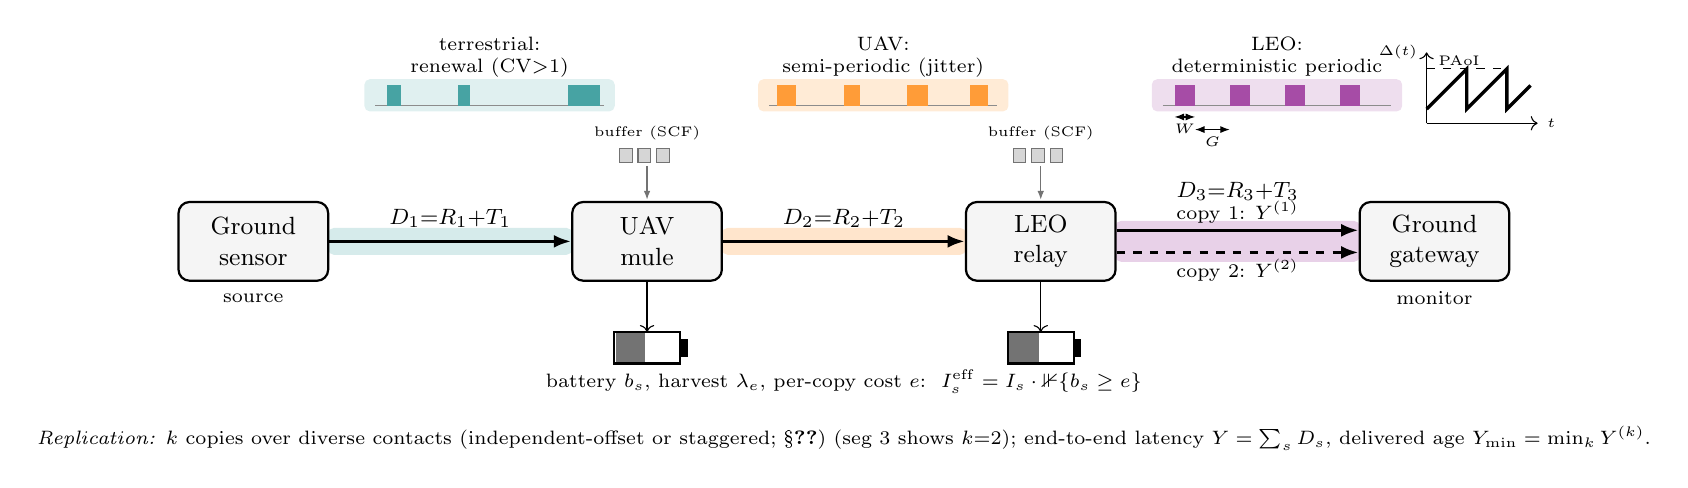
\begin{tikzpicture}[font=\small,
  station/.style={draw,thick,rounded corners,minimum width=1.9cm,
    minimum height=1.0cm,align=center,fill=black!4},
  seg/.style={-{Latex[length=2.2mm]},very thick},
  lbl/.style={font=\footnotesize,align=center}]
\colorlet{cterr}{teal}\colorlet{cuav}{orange}\colorlet{cleo}{violet}

% --- colored bands tie each segment to its contact-model strip ---
\fill[cterr!16,rounded corners=2pt] (0.95,-0.17) rectangle (4.05,0.17);
\fill[cuav!20,rounded corners=2pt]  (5.95,-0.17) rectangle (9.05,0.17);
\fill[cleo!18,rounded corners=2pt]  (10.95,-0.26) rectangle (14.05,0.26);

% --- stations ---
\node[station] (s) at (0,0)   {Ground\\sensor};
\node[station] (u) at (5,0)   {UAV\\mule};
\node[station] (l) at (10,0)  {LEO\\relay};
\node[station] (g) at (15,0)  {Ground\\gateway};
\node[lbl,font=\scriptsize] at (0,-0.72) {source};
\node[lbl,font=\scriptsize] at (15,-0.72) {monitor};

% --- segments 1,2 (single copy) ---
\draw[seg] (s) -- node[lbl,above=1pt]{$D_1{=}R_1{+}T_1$} (u);
\draw[seg] (u) -- node[lbl,above=1pt]{$D_2{=}R_2{+}T_2$} (l);

% --- segment 3 (LEO): two explicit decorrelated copies (k=2) ---
\node[lbl] at (12.5,0.63){$D_3{=}R_3{+}T_3$};
\draw[seg] ([yshift=4pt]l.east) --
  node[lbl,font=\scriptsize,above=-1.5pt]{copy 1: $Y^{(1)}$} ([yshift=4pt]g.west);
\draw[seg,dashed] ([yshift=-4pt]l.east) --
  node[lbl,font=\scriptsize,below=-1.5pt]{copy 2: $Y^{(2)}$} ([yshift=-4pt]g.west);

% --- store-carry-forward buffers at the relays ---
\foreach \x in {5,10}{
  \foreach \i in {0,1,2}{\fill[black!16,draw=black!55]
    ({\x-0.35+0.235*\i},1.0) rectangle ({\x-0.19+0.235*\i},1.18);}
  \node[lbl,font=\tiny] at (\x,1.37){buffer (SCF)};
  \draw[-{Latex[length=1.1mm]},thin,black!55] (\x,0.96)--(\x,0.53);
}

% --- color-coded ON/OFF schedule strips (contact models) ---
\begin{scope}[shift={(1.55,1.72)}]
  \fill[cterr!12,rounded corners=2pt] (-0.14,-0.07) rectangle (3.04,0.34);
  \draw[thin,black!45] (0,0)--(2.9,0);
  \foreach \a/\b in {0.15/0.32,1.05/1.2,2.45/2.85}{\fill[cterr!72] (\a,0) rectangle (\b,0.26);}
  \node[lbl,font=\scriptsize] at (1.45,0.62){terrestrial:\\renewal (CV$>$1)};
\end{scope}
\begin{scope}[shift={(6.55,1.72)}]
  \fill[cuav!16,rounded corners=2pt] (-0.14,-0.07) rectangle (3.04,0.34);
  \draw[thin,black!45] (0,0)--(2.9,0);
  \foreach \a/\b in {0.1/0.34,0.95/1.15,1.75/2.02,2.55/2.78}{\fill[cuav!78] (\a,0) rectangle (\b,0.26);}
  \node[lbl,font=\scriptsize] at (1.45,0.62){UAV:\\semi-periodic (jitter)};
\end{scope}
\begin{scope}[shift={(11.55,1.72)}]
  \fill[cleo!13,rounded corners=2pt] (-0.14,-0.07) rectangle (3.04,0.34);
  \draw[thin,black!45] (0,0)--(2.9,0);
  \foreach \x in {0.15,0.85,1.55,2.25}{\fill[cleo!70] (\x,0) rectangle ({\x+0.26},0.26);}
  \node[lbl,font=\scriptsize] at (1.45,0.62){LEO:\\deterministic periodic};
  \draw[{Latex[length=1.2mm]}-{Latex[length=1.2mm]}] (0.15,-0.14)--(0.41,-0.14);
  \node[font=\tiny,below=-1pt] at (0.28,-0.14){$W$};
  \draw[{Latex[length=1.2mm]}-{Latex[length=1.2mm]}] (0.41,-0.30)--(0.85,-0.30);
  \node[font=\tiny,below=-1pt] at (0.63,-0.30){$G$};
\end{scope}

% --- batteries / energy gate at relays ---
\foreach \x in {5,10}{
  \draw[thick] (\x-0.42,-1.55) rectangle (\x+0.42,-1.15);
  \draw[thick,fill=black] (\x+0.42,-1.45) rectangle (\x+0.5,-1.25);
  \fill[black!55] (\x-0.4,-1.53) rectangle (\x-0.02,-1.17);
  \draw[->,thin] (\x,-0.5)--(\x,-1.15);
}
\node[lbl,font=\scriptsize] at (7.5,-1.78)
  {battery $b_s$, harvest $\lambda_e$, per-copy cost $e$:\ \ $I^{\mathrm{eff}}_s=I_s\cdot\mathbb{1}\{b_s\ge e\}$};

% --- replication note (centred on the chain midpoint x=7.5) ---
\node[lbl,font=\scriptsize,align=center] at (7.5,-2.5)
  {\emph{Replication:} $k$ copies over diverse contacts (independent-offset or staggered; \S\ref{sec:r3}) (seg~3 shows
   $k{=}2$);\ end-to-end latency $Y=\sum_s D_s$, delivered age
   $Y_{\min}=\min_k Y^{(k)}$.};

% --- AoI sawtooth inset at the monitor ---
\begin{scope}[shift={(14.9,1.5)},scale=0.6]
  \draw[->] (0,0)--(2.35,0) node[right,font=\tiny]{$t$};
  \draw[->] (0,0)--(0,1.5) node[left,font=\tiny]{$\Delta(t)$};
  \draw[very thick] (0,0.3)--(0.85,1.15)--(0.85,0.3)--(1.7,1.15)--(1.7,0.3)--(2.2,0.8);
  \draw[dashed,thin] (0,1.15)--(1.7,1.15);
  \node[font=\tiny,anchor=west] at (0.05,1.32){PAoI};
\end{scope}
% balance the bounding box about the chain centre so the diagram is centred
\path (-1.7,0) (16.7,0);
\end{tikzpicture}}
\caption{System model. A status source (ground sensor) reaches the
monitor (ground gateway) over an ordered chain of \emph{scheduled,
intermittently available} segments---terrestrial opportunistic, UAV
mule, LEO relay---each a store-carry-forward server (bundles wait in a
buffer) that is ON only during contact windows. The color-coded
per-segment ON/OFF pattern differs by segment type (high-variance renewal,
semi-periodic with jitter, deterministic periodic), so a bundle generated
mid-gap ages for a residual wait $R_s$ before a service+propagation
$T_s$, giving increment $D_s=R_s+T_s$ and end-to-end latency
$Y=\sum_s D_s$. Bundles are \emph{replicated} over $k$ \emph{diverse}
contacts---independent-offset or deterministically staggered, two
distinct regimes treated separately in Section~\ref{sec:r3} (independent
offsets give independent residuals; staggered fixed plans give
negatively dependent ones; distinct router next-hops guarantee
neither). Segment~3 illustrates $k{=}2$ with
copies $Y^{(1)},Y^{(2)}$ and delivered age $Y_{\min}=\min_k Y^{(k)}$. A
finite energy-harvesting battery at each relay gates its usable contacts,
$I^{\mathrm{eff}}_s=I_s\cdot\mathbb{1}\{b_s\ge e\}$.
The monitor tracks the Age of Information $\Delta(t)$ and its peak (PAoI).}
\label{fig:model}
\end{figure*}

A status source delivers updates to a remote monitor over an ordered
chain of $S$ store-carry-forward segments, indexed $s=1,\dots,S$. In the
canonical instance (Fig.~\ref{fig:model}), a ground sensor reaches a
ground gateway through a UAV mule and a LEO relay---the sensor acting as
the source and the gateway as the monitor---so the path is ground
sensor~$\to$~UAV~$\to$~LEO~$\to$~ground gateway. Each segment is a server
whose availability is dictated by a contact schedule rather than being
continuous.

\paragraph*{Per-segment contact abstraction}
\begin{itemize}
\item \emph{LEO}: deterministic periodic ON/OFF, window $W_s$ once per
period $P_s$ (Section~\ref{sec:r1});
\item \emph{UAV}: semi-periodic / jittered renewal ON/OFF (reduces to
the LEO case as jitter $\to 0$; genuinely Markov-modulated schedules,
with correlated successive gaps, are an extension);
\item \emph{Terrestrial}: stochastic renewal ON/OFF.
\end{itemize}

\paragraph*{Quantities and the freshness metrics}
$\AoI(t)=t-g^{\star}(t)$ is the AoI at the monitor, where $g^{\star}(t)$
is the generation time of the freshest \emph{delivered} bundle; it drifts
up at unit rate and resets whenever a delivery brings fresher
information (a stale or duplicate copy causes no reset). Intermittent
gating supports two distinct traffic models, and their peak-age
processes differ---so we define \emph{three} peak quantities and state,
for every result, which one it characterizes
(Fig.~\ref{fig:metric}):
\begin{itemize}
\item \emph{per-reset} $\PAoI$ (textbook): the average of the age just
before \emph{every} reset. When a window delivers a back-to-back burst
of updates it also counts the small intra-burst peaks, deflating the
average;
\item \emph{outage-peak age} $\OPAoI$: the average, over contact
cycles, of the maximum age just before that contact's deliveries---the
worst-case staleness per silent gap. Under \emph{generate-at-will}
traffic (fresh data available at every window) the single-LEO cycle
peak is $\OPAoI=T_s+G$ (Section~\ref{sec:r1});
\item \emph{per-update} $\PAoIper$: the standard PAoI when the source
launches one update per firing epoch (paced generation): each update
yields one reset, and $\E[\PAoIper]=\E[Z]+\E[\Ymin]$ with $Z$ the
inter-firing interval and $\Ymin$ the delivered latency. Here per-reset
and per-update coincide. The identity presumes deliveries
\emph{preserve generation order}: if a newer update overtakes an older
one, the older delivery arrives stale and resets nothing. Order
preservation is guaranteed whenever the latency spread is bounded by
the firing interval, $Y_{\max}-Y_{\min}\le Z_{\min}$ (with
lattice-supported $Z$ and bounded $Y$ this is checkable from the plan;
note $\sum_s G_s$ can exceed the firing interval on long multi-segment
paths, where the condition binds). When it fails, $\PAoIper$ must be
evaluated over the subsequence of \emph{freshness-resetting}
deliveries, and $\E[Z]+\E[\Ymin]$ no longer generally characterizes
\emph{or bounds} that process: consecutive resets can sit several
firing intervals apart while the resetting updates are the atypically
fast ones, so the true peak can land on either side (e.g.\
deterministic $Z{=}1$ with repeating latencies $4,3,2,0,5$ resets once
per five epochs with peak $5>\E[Z]{+}\E[Y]{=}3.8$).
\end{itemize}
These are genuinely different processes: for $P{=}1$, $W{=}0.1$,
$T_s{\approx}0$, $\OPAoI=0.9$ while $\E[\PAoIper]=1.405$
($=P+\E[R]$)---neither is an approximation of the other.
Results~1 and the renewal generalization characterize $\OPAoI$ (and
time-average AoI); Results~2--3, the tail corollary, and the policy
characterize $\PAoIper$ under paced generation. Our Tier-2
reconstruction clusters resets within one contact window and keeps the
burst maximum, i.e.\ it measures $\OPAoI$
(Section~\ref{sec:sim}); the Tier-1 Result-3 simulations measure
$\PAoIper$. For a single copy, the per-segment latency
increment is $D_s=R_s+T_s$ with $R_s$ the residual wait and $T_s$ the
lumped (near-deterministic) service plus propagation, and the end-to-end
latency is $Y=\sum_{s=1}^S D_s$; with replication degree $k$ the delivered
latency is $\Ymin=\min(Y^{(1)},\dots,Y^{(k)})$.

\paragraph*{Uncongested-contact regime (scope)}
Throughout, a contact is usable the instant it opens and $T_s$ absorbs
transmission and propagation: we work in the \emph{low-load} regime
where contact capacity (window duration $\times$ rate) exceeds the
offered bundle volume, so residual waits---hours---dominate service
times---seconds---and replication's second cost, \emph{contact volume},
is negligible next to its energy cost. Status updates sit deep in this
regime (our Iridium scenario uses ${\sim}10^{-5}$ of a window per
update), but the assumption is load-bearing: near contact capacity,
in-window queueing, overbooking~\cite{bezirgiannidis}, and the volume
of extra copies re-enter. Section~\ref{sec:sim} measures the boundary.

\begin{figure}[t]
\centering
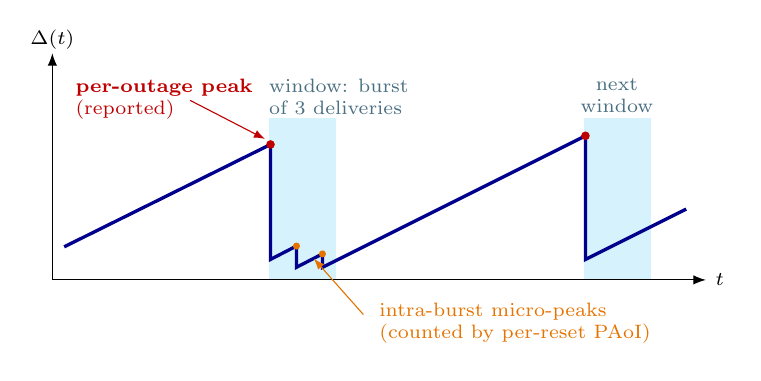
\begin{tikzpicture}[font=\footnotesize,x=1cm,y=1cm,
  note/.style={font=\scriptsize,align=center}]
\colorlet{cwin}{cyan!16}\colorlet{cage}{blue!55!black}
\colorlet{cpk}{red!75!black}\colorlet{cmicro}{orange!90!black}
% contact windows (shaded)
\fill[cwin] (2.6,0) rectangle (3.45,2.05);
\fill[cwin] (6.6,0) rectangle (7.45,2.05);
\node[note,cyan!45!black,anchor=north west,align=left] at (2.48,2.68)
  {window: burst\\of 3 deliveries};
\node[note,cyan!45!black,anchor=north] at (7.02,2.68) {next\\window};
% axes
\draw[-{Latex[length=1.6mm]}] (-0.15,0)--(8.15,0) node[right,font=\scriptsize]{$t$};
\draw[-{Latex[length=1.6mm]}] (-0.15,0)--(-0.15,2.88)
  node[above,font=\scriptsize,inner sep=1pt]{$\AoI(t)$};
% sawtooth: gap ramp, burst of 3 resets in window, gap ramp, reset
\draw[very thick,cage]
 (0,0.42)--(2.62,1.72)--(2.62,0.26)--(2.95,0.43)--(2.95,0.16)
 --(3.28,0.33)--(3.28,0.16)--(6.62,1.83)--(6.62,0.26)--(7.9,0.9);
% outage peaks (dots + label placed in the free upper-left area)
\fill[cpk] (2.62,1.72) circle (0.055);
\fill[cpk] (6.62,1.83) circle (0.055);
\node[note,cpk,anchor=north west,align=left] at (0.02,2.68)
  {\textbf{per-outage peak}\\(reported)};
\draw[-{Latex[length=1.4mm]},cpk] (1.60,2.28) -- (2.55,1.79);
% micro peaks annotated below the axis (keeps the curve clear)
\fill[cmicro] (2.95,0.43) circle (0.045);
\fill[cmicro] (3.28,0.33) circle (0.045);
\draw[-{Latex[length=1.4mm]},cmicro] (3.80,-0.44) -- (3.17,0.27);
\node[note,cmicro,anchor=west,align=left] at (3.88,-0.55)
  {intra-burst micro-peaks\\(counted by per-reset PAoI)};
\end{tikzpicture}
\caption{The peak-age taxonomy. A contact window delivers a back-to-back
burst of distinct updates; each fresher delivery resets the age. The
textbook \emph{per-reset} $\PAoI$ also averages the small intra-burst
peaks, deflating the mean; the \emph{outage peak} $\OPAoI$ keeps only
the burst maximum---the conservative cycle-level statistic (within
each cycle it dominates every intra-burst peak; with variable burst
sizes the two \emph{averages} need not order). Under paced
generation (one update per firing epoch) each update yields one reset
and the per-update peak $\PAoIper=Z+\Ymin$ applies; the three coincide
when each contact delivers exactly one update.}
\label{fig:metric}
\end{figure}

\paragraph*{Energy coupling}
Battery $b_s(t)$, harvest rate $\lambda_{e,s}$, per-copy energy $e$. The
effective availability is $I^{\mathrm{eff}}_s(t)=I_s(t)\cdot
\ind\{b_s(t)\ge e\}$: energy scarcity thins contacts (stretches the
residual wait) and replication draws the battery down faster (starving
future contacts). This tension is resolved in
Sections~\ref{sec:r3}--\ref{sec:r3hard}. \emph{Scope:} although the
model admits a battery per segment, the threshold analysis of
Sections~\ref{sec:r3}--\ref{sec:r3hard} adopts a \textbf{single
energy-bottleneck abstraction}---one battery (the source-side or
tightest node) gates copy launches at constant per-copy cost $e$, the
binding constraint in our scenarios. Route-dependent costs and
interacting per-relay batteries are an extension we do not claim
(Section~\ref{sec:sim} gates energy at the source accordingly).

\begin{remark}[Report both metrics]
Exact average AoI in tandems is closed-form only to two--three hops,
while the peak metrics remain reachable; and under intermittency
$\OPAoI$ can fall \emph{below} time-average AoI
(Remark~\ref{rem:inversion}), so we report peak and average
throughout.
\end{remark}

\begin{table}[t]
\caption{Notation.}
\label{tab:notation}
\centering
\renewcommand{\arraystretch}{1.12}
\setlength{\tabcolsep}{4pt}
\footnotesize
\begin{tabular}{ll}
\hline
$P,\,W,\,G$ & contact period, window, silent gap $G=P-W$ \\
$\delta$ & duty cycle $W/P$;\; $\dutyeff=\delta\peff$ usable-ON fraction \\
$U$ & arrival phase (Sec.~\ref{sec:r1}); ON duration (Sec.~\ref{sec:renewal}) \\
$V,\,C$ & OFF gap, renewal cycle $C=U+V$ (Sec.~\ref{sec:renewal}) \\
$R_s,\,T_s$ & residual wait; service$+$propagation at segment $s$ \\
$D_s,\,Y$ & increment $R_s{+}T_s$; end-to-end latency $\sum_s D_s$ \\
$k,\,\Ymin$ & replication degree; delivered latency $\min_k Y^{(k)}$ \\
$Z,\,\AoI$ & inter-firing interval; age at the monitor \\
$\OPAoI,\,\PAoIper$ & outage-peak age; per-update peak age \\
$b_s,\,B,\,e$ & battery level, capacity, per-copy energy cost \\
$\lambda_e,\,\eta$ & harvest rate; energy adequacy $\lambda_e P/e$ \\
$\peff,\,L$ & usable-window probability; cap-overflow loss \\
$\mathcal{A}(k),\,\kstar$ & mean-$\PAoIper$ objective \eqref{eq:obj}; optimal degree \\
$K_{\max}$ & candidate copy routes / contact opportunities \\
\hline
\end{tabular}
\end{table}

\begin{table}[t]
\caption{Modeling assumptions and their failure modes.}
\label{tab:assumptions}
\centering
\renewcommand{\arraystretch}{1.2}
\begin{tabular}{p{2.5cm}p{1.1cm}p{3.3cm}}
\hline
Assumption & Where & If violated \\
\hline
Decorrelated contacts per copy & Results 2--3 & same-bottleneck copies: gain $\to 0$ \\
Random offsets / spread-out delays & Lem.~\ref{lem:mix}, Rem.~\ref{rem:fixedmix} & commensurate or lattice: locking \\
$k\le 2$ closed form & Result 2 & general $k$ via $\int(1-F_Y)^k$ (numerical) \\
Generate-at-will & Result 1 & finite $\lambda$: $+1/\lambda$ floor (Sec.~\ref{sec:renewal}) \\
Large battery & Result 3 (fluid $\peff$) & finite $B$: $\peff\le\min(1,\eta/k)$, presses $\kstar$ down \\
\hline
\end{tabular}
\end{table}

% =====================================================================
\section{Result 1: Residual-Wait Laws for Scheduled
Contacts}\label{sec:r1}
A LEO satellite rises over the ground terminal once per orbital period
$P$ and stays in view for a contact window of duration $W$; the link is
therefore ON during $[0,W)$ of each period and OFF (dark) during the
silent gap $G\triangleq P-W$ that follows, so the terminal is in contact
only a fraction $\delta\triangleq W/P$ of the time---the duty cycle
(Fig.~\ref{fig:r1def}). A status update generated at a stationary
(random-phase) instant meets this schedule at a uniformly random phase $U\sim\mathrm{Unif}[0,P)$
(justified by Lemma~\ref{lem:mix}): if $U$ falls inside a window the
bundle is forwarded at once, otherwise it must age in buffer until the
next pass. This residual wait is
\begin{equation}
R=\begin{cases}0,& U\in[0,W)\\ P-U,& U\in[W,P)\end{cases}
\end{equation}
a mixed law with atom $\Prob(R=0)=W/P$ and uniform slab $f_R(r)=1/P$ on
$(0,G]$; $\Prob(R>r)=(G-r)/P$ on $[0,G]$, $R_{\max}=G$.

\begin{figure}[t]
\centering
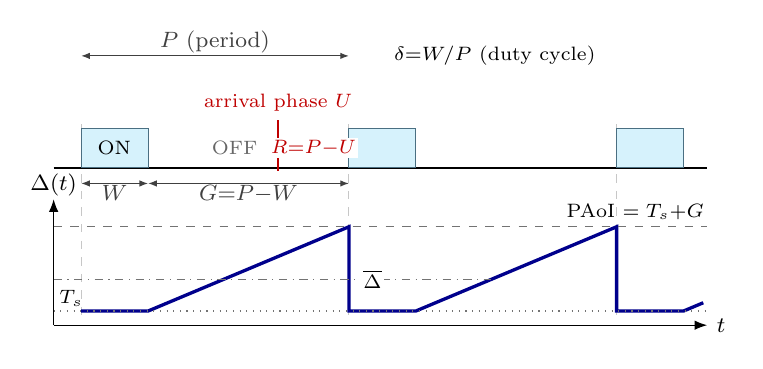
\begin{tikzpicture}[font=\footnotesize,x=1cm,y=1cm,
  win/.style={fill=cyan!16,draw=cyan!45!black,thin},
  ax/.style={-{Latex[length=1.6mm]}},
  dim/.style={{Latex[length=1.1mm]}-{Latex[length=1.1mm]},black!75}]
\colorlet{cage}{blue!55!black}\colorlet{carr}{red!75!black}
% vertical guides at window openings (link schedule to AoI)
\foreach \x in {0,3.4,6.8}{\draw[dashed,black!22] (\x,2.55)--(\x,0.02);}
% ===== schedule panel (link ON/OFF) =====
\draw[thick] (-0.35,2.0)--(7.95,2.0);
\foreach \x in {0,3.4,6.8}{\fill[win] (\x,2.0) rectangle (\x+0.85,2.5);}
\node[font=\scriptsize] at (0.42,2.25){ON};
\node[font=\scriptsize,black!60] at (1.95,2.25){OFF};
% period / duty-cycle dimensions raised clear of the arrival annotation
\draw[dim] (0,3.42)--(3.4,3.42) node[midway,above,inner sep=1pt]{$P$ (period)};
\node[font=\scriptsize,anchor=west] at (3.85,3.42){$\delta{=}W/P$ (duty cycle)};
% W and G on one line beneath the bar
\draw[dim] (0,1.80)--(0.85,1.80) node[midway,below,inner sep=0.5pt]{$W$};
\draw[dim] (0.85,1.80)--(3.4,1.80) node[midway,below,inner sep=0.5pt]{$G{=}P{-}W$};
% arrival + residual wait
\draw[thick,carr] (2.5,1.96)--(2.5,2.60);
\node[font=\scriptsize,carr,anchor=south,inner sep=1.5pt] at (2.5,2.66){arrival phase $U$};
\draw[dim,carr] (2.5,2.25)--(3.4,2.25);
\node[font=\scriptsize,carr,fill=white,inner sep=0.8pt] at (2.95,2.25){$R{=}P{-}U$};
% ===== AoI panel: sawtooth Delta(t) =====
\draw[ax] (-0.35,0)--(7.95,0) node[right]{$t$};
\draw[ax] (-0.35,0)--(-0.35,1.60) node[above,inner sep=1pt]{$\Delta(t)$};
\draw[very thick,cage]
  (0,0.18)--(0.85,0.18)--(3.4,1.25)--(3.4,0.18)--(4.25,0.18)--(6.8,1.25)
  --(6.8,0.18)--(7.65,0.18)--(7.9,0.285);
\draw[dashed,black!55] (-0.35,1.25)--(7.95,1.25);
\node[font=\scriptsize,anchor=east,inner sep=1pt] at (7.95,1.44){PAoI $=T_s{+}G$};
\draw[dashdotted,black!55] (-0.35,0.58)--(5.2,0.58);
\node[font=\scriptsize,anchor=west,fill=white,inner sep=0.8pt] at (3.55,0.58){$\overline{\Delta}$};
\draw[dotted,black!55] (-0.35,0.18)--(7.95,0.18);
\node[font=\scriptsize,anchor=west,inner sep=1pt] at (-0.32,0.34){$T_s$};
\end{tikzpicture}
\caption{Result~1 parameters. \emph{Top:} the LEO segment is ON for a
window $W$ once per period $P$ (silent gap $G{=}P{-}W$, duty cycle
$\delta{=}W/P$); a bundle generated at arrival phase $U$ in the gap waits
a residual $R{=}P{-}U$ for the next window. \emph{Bottom:} the resulting
age $\Delta(t)$ is pinned near the service+propagation floor $T_s$ during
a window and ramps over the gap, peaking at $\OPAoI{=}T_s{+}G$; the
time-average is $\overline{\Delta}{=}T_s{+}(P{-}W)^2/2P$
(Theorem~\ref{thm:r1}).}
\label{fig:r1def}
\end{figure}

\begin{theorem}[LEO AoI/OPAoI anchor]\label{thm:r1}
With service$+$propagation $T_s$,
\begin{align}
\E[R]&=\frac{(P-W)^2}{2P}=\tfrac{P}{2}(1-\delta)^2,\quad
\E[R^2]=\frac{G^3}{3P},\\
\overline{\AoI}_{\mathrm{LEO}}&=T_s+\tfrac{P}{2}(1-\delta)^2,\qquad
\OPAoI_{\mathrm{LEO}}=T_s+P(1-\delta).
\end{align}
\end{theorem}
The law itself is classical residual-life theory, stated as the anchor
on which the DTN-specific structure builds. Note the provisioning
consequence: sparse contacts hurt the mean age \emph{quadratically} in
$(1-\delta)$ but the peak only \emph{linearly}, so mean- and
peak-optimal contact provisioning differ.

\paragraph*{Energy-thinning bridge}
If each window is usable with probability $\peff$ (battery $\ge e$),
i.i.d.\ across periods, the usable schedule is again alternating-renewal
with OFF gap $V'=(J{-}1)P+G$, $J\sim\mathrm{Geom}(\peff)$, so every
closed form extends through the renewal law of
Section~\ref{sec:renewal} with $V\to V'$; in particular the exact
thinned residual is
\begin{equation}\label{eq:thin}
\E[R_{\mathrm{eff}}]=
\underbrace{\frac{(P-W)^2}{2P}}_{\text{contact gating}}
+\underbrace{P\,\frac{1-\peff}{\peff}}_{\text{energy thinning}}
-\underbrace{\frac{(1-\peff)W^2}{2P}}_{O(\delta^2)} .
\end{equation}
We caution that this is a \emph{thinning}, not a rescaling: the
shorthand $\dutyeff=\delta\peff$ preserves only the long-run usable-ON
fraction, and substituting $\delta\mapsto\delta\peff$ into the
Theorem~\ref{thm:r1} forms does \emph{not} reproduce
\eqref{eq:thin}---skipped windows cluster the silence into whole
periods, which the residual's second-moment dependence
($\E[V'^2]/2\E[C']$) captures and a duty-cycle rescaling does not. The
i.i.d.\ premise itself is a mean-field approximation---a finite battery
correlates consecutive windows---made precise in
Section~\ref{sec:r3hard}.

% =====================================================================
\subsection{Renewal Generalization: UAV and Terrestrial
Segments}\label{sec:renewal}
Real UAV and terrestrial links are not perfectly periodic: a UAV mule
revisits the sensor field on a jittered patrol, and opportunistic
terrestrial contacts appear at random. One \emph{alternating-renewal}
model captures all three segment types---with the deterministic LEO
schedule as a special case---by letting each contact cycle be an ON
period of duration $U$ (the window) followed by an OFF gap of duration
$V$ (mean $G$, the dark interval before the next contact), where $U$ and
$V$ may now be random; the cycle length is $C=U+V$ and the duty cycle is
$\delta=\mathbb E[U]/\mathbb E[C]$. By renewal-reward and the inspection
paradox, a stationary arrival sees
\begin{equation}\label{eq:renewal}
\begin{aligned}
\Pr(R{=}0)&=\delta,\qquad f_R(r)=\frac{\Pr(V>r)}{\mathbb E[C]},\\
\E[R]&=\frac{\E[V^2]}{2\,\E[C]},\qquad \E[\OPAoI]=T_s+\E[V].
\end{aligned}
\end{equation}
Deterministic $V$ recovers Theorem~\ref{thm:r1} (LEO); a low-variance $V$
models UAV semi-periodic jitter ($\to$ LEO as the jitter vanishes);
exponential $V$ is the 2-state CTMC (the ``unreliable-server'' case, here
a special case rather than the contribution); heavy-tailed $V$ models
opportunistic terrestrial contacts.

\begin{remark}[AoI/PAoI inversion]\label{rem:inversion}
Mean $\OPAoI$ depends only on $\E[V]$ while mean AoI grows with the gap
variance, so
$\E[\OPAoI]<\overline{\AoI}\iff \E[V^2]>2\E[C]\E[V]$. Writing
$C=U+V$, this is exactly
\begin{equation}\label{eq:invcond}
\mathrm{CV}^2(V)>1+\frac{2\,\E[U]}{\E[V]},
\end{equation}
which reduces to the familiar $\mathrm{CV}^2(V)>1$ only in the sparse-duty
limit $\delta\to0$ ($\E[U]/\E[V]\to0$); for the plotted parameters
($\E[U]/\E[V]=1/9$) the threshold is $\mathrm{CV}^2\approx1.22$, i.e.\
$\mathrm{CV}\approx1.11$. Peak age can therefore sit
\emph{below} average age on heavy-tailed terrestrial links
(Fig.~\ref{fig:inversion}) -- a single freshness number is misleading
across heterogeneous segments. The order-statistic replication analysis below acts on the residual
law abstractly; the energy-threshold structure extends when the
resulting gain profile and firing process satisfy the conditions of
Section~\ref{sec:r3}.
\end{remark}

% =====================================================================
\section{Result 2: Phase Mixing and Two-Copy PAoI}\label{sec:r2}
Composing segments needs care. The residual wait $R_s$ a bundle incurs at
segment $s$ depends on \emph{when} it reaches that segment relative to the
segment's own schedule---its arrival phase---which is itself displaced by
all the upstream delays. Writing the phase as
$\Phi_s=\bigl(g+\sum_{j<s}D_j\bigr)\bmod P_s$ (generation time $g$ plus the
accumulated increments, reduced modulo the segment period $P_s$), $R_s$ is
therefore not automatically independent of the upstream increments
$\{D_j\}_{j<s}$, and the per-segment delays cannot simply be added. The
following lemma gives the condition under which they can.

\begin{lemma}[Uniform phases under random offsets]\label{lem:mix}
Let each segment's schedule carry an offset $\Theta_s\sim
\mathrm{Unif}[0,P_s)$, independent across segments and of the
generation process (the \emph{random-offset ensemble}). Then the phases
$\{\Phi_s\}$ are exactly uniform and mutually independent; hence
$\{D_s\}$ are independent, the aged-update correction vanishes, and
$f_Y=f_{D_1}\ast\cdots\ast f_{D_S}$.
\end{lemma}
\begin{proof}
$\Phi_s=(g+\sum_{j<s}D_j-\Theta_s)\bmod P_s$; conditioning on the
generation time and all upstream increments, the wrap of an independent
uniform $\Theta_s$ is uniform on $[0,P_s)$ and independent of the
conditioning variables and of the other $\Theta_j$.
\end{proof}

\begin{remark}[Fixed plans: two asymptotic mechanisms, one
approximation]\label{rem:fixedmix}
For one \emph{fixed} plan (deterministic offsets), uniformity and
independence are not automatic; they arise in two limits whose limiting
parameter we now name explicitly.
(a)~\emph{Horizon limit, deterministic Weyl.} Under paced generation at
spacing $\GEN$ with $\GEN/P_1$ irrational, the \emph{first-segment}
phase sequence $n\,\GEN\bmod P_1$ equidistributes over the first $n$
updates as $n\to\infty$ (Weyl)---this part is rigorous, and it is what
justifies the uniform-arrival marginal on the entry segment of a fixed
plan. We stress its limit: a \emph{downstream} phase is not linear in
$n$---it is the generation epoch pushed through the composed
store-carry-forward map, whose increments are themselves determined by
the upstream schedules---and joint equidistribution of the
\emph{generation} phases does not by itself imply statistical
independence of the downstream residuals. We do not prove
measure-preservation for the composed contact map; downstream
decoupling on fixed plans rests on mechanism (b) or on measurement.
(b)~\emph{Convolution limit, spread-out delays.} If the upstream sum
$\sum_{j<s}D_j$ of $m$ random increments has a spread-out (non-lattice)
component, its characteristic function satisfies
$|\E\,e^{2\pi i n\Sigma/P_s}|\to0$ as $m\to\infty$ for all $n\ne0$, so
the wrapped phase of a \emph{single} update converges to uniform with
hop depth---this gives the uniform \emph{marginal} at segment $s$;
mutual independence across segments is again the measured part. Large
dispersion \emph{alone} is not sufficient: a
lattice-valued sum concentrated on multiples of $P_s$ has arbitrarily
large variance yet a degenerate wrapped phase.
At any finite horizon and hop count the fixed-plan use of the uniform
law is therefore an \emph{engineering approximation}, whose accuracy we
measure rather than assume: KS-to-uniform $0.001$ in the fixed-plan
simulations, per-seed composition error $\le5.9\%$ on the heterogeneous
chain, and---as the cautionary bound---real Iridium pairs whose
residual correlations range from $-0.51$ to $+0.88$ when condition (a)
is violated by near-commensurate passes
(Section~\ref{sec:sim}). The named failure modes are (a$'$)
commensurate periods (a UAV synchronized to one specific LEO pass) and
(b$'$) lattice-concentrated upstream delays
(Fig.~\ref{fig:mixing}); Lemma~\ref{lem:mix} (random offsets) remains
the exact statement.
\end{remark}

\begin{figure}[t]
\centering
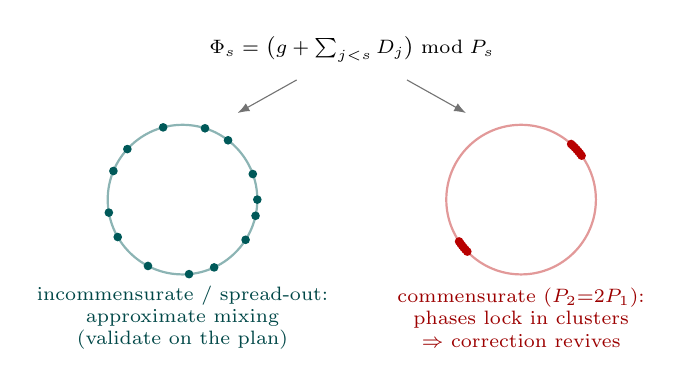
\begin{tikzpicture}[font=\footnotesize,x=1cm,y=1cm]
\colorlet{cmix}{teal!70!black}\colorlet{clock}{red!72!black}
% ---- left wheel: incommensurate -> equidistributed phases ----
\draw[thick,cmix!45] (0,0) circle (0.95);
\foreach \i in {0,...,13}{
  \fill[cmix] ({0.95*cos(137.5*\i)},{0.95*sin(137.5*\i)}) circle (0.055);}
\node[font=\scriptsize,align=center,cmix!80!black] at (0,-1.5)
  {incommensurate / spread-out:\\approximate mixing\\(validate on the plan)};
% ---- right wheel: commensurate -> locked phases ----
\begin{scope}[shift={(4.3,0)}]
\draw[thick,clock!40] (0,0) circle (0.95);
\foreach \a in {38,42,46,40,44,36,48}{
  \fill[clock] ({0.95*cos(\a)},{0.95*sin(\a)}) circle (0.055);}
\foreach \a in {216,220,224,218,222,214}{
  \fill[clock] ({0.95*cos(\a)},{0.95*sin(\a)}) circle (0.055);}
\node[font=\scriptsize,align=center,clock!85!black] at (0,-1.5)
  {commensurate ($P_2{=}2P_1$):\\phases lock in clusters\\$\Rightarrow$ correction revives};
\end{scope}
% phase annotation raised clear of both wheels; arrows start below it
\node[font=\scriptsize,align=center,anchor=south] at (2.15,1.62)
  {$\Phi_s=\bigl(g+\textstyle\sum_{j<s}D_j\bigr)\bmod P_s$};
\draw[-{Latex[length=1.5mm]},black!55] (1.45,1.52) -- (0.70,1.10);
\draw[-{Latex[length=1.5mm]},black!55] (2.85,1.52) -- (3.60,1.10);
\end{tikzpicture}
\caption{Phase mixing (Lemma~\ref{lem:mix},
Remark~\ref{rem:fixedmix}). The arrival phase at
segment $s$ lives on a circle of circumference $P_s$. Under random
schedule offsets the wrapped phase is exactly uniform and independent
of the upstream increments; for a fixed plan with spread-out
(non-lattice) upstream delays and incommensurate periods the same
decoupling holds \emph{approximately} (left)---the regime in which
latencies compose by
convolution. Commensurate periods lock the phase into clusters (right):
the failure mode of a UAV synchronized to one specific LEO pass.}
\label{fig:mixing}
\end{figure}

Under paced generation with order-preserving deliveries
(Section~\ref{sec:model}; $Y_{\max}-Y_{\min}\le Z_{\min}$ suffices),
$\PAoIper=Z+Y$ and the single-copy mean needs no independence:
\begin{equation}
\E[\PAoIper{}^{(1)}]=\E[Z]+\sum_{s=1}^S(\E[R_s]+T_s),
\end{equation}
with deterministic envelope $\PAoIper{}^{(1)}\le Z_{\max}+\sum_s(G_s+T_s)$.

\begin{theorem}[$k{=}2$ per-update PAoI, phase-mixing regime]\label{thm:r2}
With i.i.d.\ copy latencies $Y^{(1)},Y^{(2)}\sim F_Y$ and
$\Ymin=\min(Y^{(1)},Y^{(2)})$,
\begin{align}
\E[\PAoIper{}^{(2)}]&=\E[Z]+\int_0^\infty[1-F_Y(y)]^2\,dy,\\
\E[\Ymin]&=\E[Y]-\tfrac12\,\E\bigl|Y^{(1)}-Y^{(2)}\bigr|\le\E[Y],
\end{align}
with equality iff $Y$ is deterministic.
\end{theorem}

\begin{remark}[Cadence, dispersion, and what replication buys]
Replication leaves the \emph{generation} cadence unchanged (one reset
per \emph{delivered} update, at its earliest surviving copy; an update
losing all copies produces none), so in the lossless limit
the mean inter-delivery interval is invariant, $\E[Z']{=}\E[Z]$, and
replication acts only through $\Ymin$---whose saving is exactly half
the mean absolute difference of path latencies (the standard
Gini-mean-difference identity): largest at sparse, high-dispersion
contacts, nearly nil on near-deterministic links. The invariance is a
mean-rate statement only: with losses or reordering, replication also
\emph{tightens the distribution} of $Z$ (fewer long fault-induced
outage gaps)---indeed the Tier-2 gain (Section~\ref{sec:sim}) comes
largely from eliminating such gaps, not from $\Ymin$ alone. Shrinking
the mean cadence itself requires $k$ independent update streams, a
different energy trade.
\end{remark}

\begin{remark}[Worked ratio and general $k$]
For two ensemble-phase satellites with $Y\approx R+T_s$,
$\E[\Rmin]/\E[R]=\tfrac23(1-\delta)$---a ${\approx}33\%$ cut of the
gating term at sparse contacts (Fig.~\ref{fig:r2gain}).
$\E[Y_{\min,k}]=\int_0^\infty(1-F_Y)^k$ generalizes, but closed forms
past $k{=}2$ with multi-segment convolutions are unwieldy; we use a
recursive numerical evaluation for general $k$. The minimum identity
assumes copies traverse \emph{independent} contacts; same-bottleneck
copies give $Y^{(1)}{=}Y^{(2)}$ and zero gain.
\end{remark}

% =====================================================================
\section{Result 3: Energy--Replication Threshold}\label{sec:r3}
Replicating a bundle over several contacts lowers its delivered latency
(the freshest copy wins) but each copy drains the relay's battery, so
there is a best number of copies to send---the question this section
answers. Deterministic, common service $T_s$ is an additive constant in
the peak, so the only $k$-dependent term is the LEO gating term. The
delivered residual over $k$ contacts is, in full generality, an integral
of the \emph{joint} survival,
\begin{equation}\label{eq:rminjoint}
\E[R_{\min,k}]=\int_0^\infty\Pr\bigl(R_1>r,\dots,R_k>r\bigr)\,dr,
\end{equation}
and how it evaluates depends on the plan model---the $k$ residuals are
functions of a \emph{common} arrival instant, so they are not
automatically independent even for staggered windows:
\begin{enumerate}
\item[(i)] \emph{Random-offset ensemble.} If each
copy's schedule offset $\Theta_i$ is an independent uniform on
$[0,P)$, the wrapped phases $U-\Theta_i$
are i.i.d.\ uniform, the $R_i$ are \emph{exactly} i.i.d.\ with the
residual
law of Section~\ref{sec:r1}, and \eqref{eq:rminjoint} factorizes:
\begin{equation}\label{eq:rminprod}
\E[R_{\min,k}]=\int_0^\infty\prod_{i=1}^{k}\Pr(R_i>r)\,dr
\end{equation}
\begin{equation}\label{eq:rmink}
\qquad=\int_0^{G}\!\Bigl(\frac{G-r}{P}\Bigr)^k dr
=\frac{P(1-\delta)^{k+1}}{k+1},
\end{equation}
with $G=P(1-\delta)$. (Consistency: $k{=}1$ recovers
Theorem~\ref{thm:r1}; heterogeneous marginals use
\eqref{eq:rminprod} directly.) For a \emph{fixed} plan whose copy
routes have pairwise incommensurate periods, the relative phases drift,
and the same product form is a \emph{time-average approximation} over
the horizon---not exact independence, since all residuals share the
arrival instant (Remark~\ref{rem:fixedmix}); its accuracy is checked on
the plan, and otherwise the exact joint form \eqref{eq:rminjoint}
applies.
\item[(ii)] \emph{Fixed co-period plan.} With deterministic offsets the
joint survival must be evaluated on the plan---it is deterministic and
\emph{computable at planning time}. For $k$ windows evenly staggered by
$P/k$ the union schedule is a single comb of period $P/k$, so (with
$x_+=\max\{x,0\}$)
\begin{equation}\label{eq:rminstag}
\E[R_{\min,k}]=\frac{P}{2k}\,(1-k\delta)_+^2,
\end{equation}
\emph{better} than the ensemble value \eqref{eq:rmink}: deterministic
anti-phasing beats blind placement. Once $k\delta\ge1$ the staggered
comb covers the entire period: the residual is zero, the gain profile
is flat, and further copies cannot improve the gating term---the
smallest covering degree $\lceil1/\delta\rceil$ is the
energy-conserving choice; the threshold analysis below operates on the
strictly decreasing range $k\delta<1$.
\item[(iii)] \emph{Locked phases.} Coincident offsets give
$\E[R_{\min,k}]=\E[R]$: zero gain.
\end{enumerate}
The extremal fixed plans and the ensemble form a
reference ladder---the \emph{phase ladder}
\begin{equation}\label{eq:ladder}
\underbrace{\tfrac{P}{2k}(1-k\delta)^2}_{\text{even stagger}}
\;\le\;
\underbrace{\tfrac{P(1-\delta)^{k+1}}{k+1}}_{\text{phase-agnostic}}
\;\le\;
\underbrace{\tfrac{P}{2}(1-\delta)^2}_{\text{locked}},
\end{equation}
with equality throughout at $k{=}1$. The outer terms are the extremal
fixed plans (best and worst deterministic offsets); the middle term is
the \emph{ensemble} reference, not a separator---an individual fixed
plan lands anywhere in the outer interval, on either side of it. This
is exactly the ordering
measured on real Iridium-NEXT pairs in Section~\ref{sec:sim}
(residual-min ratio $0.41$ anti-phased, $0.61$ ensemble reference,
$0.95$ near-locked, with intermediate pairs scattered on both sides). We develop the threshold below for the
\emph{phase-agnostic} profile (i)---the operative model when copy
routes have drifting relative phases or are assigned without phase
information---and note that every structural result carries over to
profile (ii) with \eqref{eq:rminstag} in place of \eqref{eq:rmink} on
its strictly decreasing range $k\delta<1$ (beyond full coverage the
profile is flat and the smallest covering degree is optimal).

\paragraph*{Energy-adequacy ratio}
Measuring energy in copies (harvest $\rho=\lambda_e/e$ copies per unit
time, contact rate $\lambda_c=1/P$), define
\begin{equation}
\eta\triangleq\frac{\rho}{\lambda_c}=\frac{\lambda_e P}{e}
=\frac{\lambda_e/\lambda_c}{e}\quad\text{(copies harvested per period).}
\end{equation}
Demanding $k$ copies per period caps the launchable fraction of update
epochs at $\peff(k)=\min(1,\eta/k)$ (flow balance; derived exactly in
Section~\ref{sec:r3hard}). Under paced generation with all-or-nothing
firing the mean per-update peak is
$\E[\PAoIper]=P/\peff+\E[R_{\min,k}]+T_s$ (a firing every $1/\peff$
periods on average, plus the delivered residual); dropping the
$k$-independent constant $P+T_s$ gives the
mean-$\PAoIper$ gating objective
\begin{equation}\label{eq:obj}
\boxed{\mathcal{A}(k)=
\underbrace{P\,\frac{1-\peff(k)}{\peff(k)}}_{\text{starvation}}
+\underbrace{\frac{P(1-\delta)^{k+1}}{k+1}}_{\text{gain}}}
,\;\peff(k)=\min\!\Bigl(1,\tfrac{\eta}{k}\Bigr).
\end{equation}
For $k\le\eta$ the starvation term vanishes and $\mathcal{A}$ is strictly
decreasing; for $k>\eta$ the starvation term equals
$\frac{P}{\eta}(k-\eta)$ and rises linearly while the gain term decays.
Hence $\mathcal{A}$ is unimodal and its minimizer is one of the two
integers bracketing $\eta$:
\begin{equation}\label{eq:kstar}
\boxed{\;\kstar=\min\!\bigl(K_{\max},\,k^{\circ}\bigr),\quad
k^{\circ}\in\{\lfloor\eta\rfloor,\lceil\eta\rceil\},\quad
\eta=\tfrac{\lambda_e P}{e}.\;}
\end{equation}
Here $\lfloor\eta\rfloor$ is the largest degree that incurs \emph{no}
starvation---the conservative DTN-reliability rule---while the skip-aware
optimum takes the extra copy, $k^{\circ}{=}\lceil\eta\rceil$, iff its
added starvation is repaid by the order-statistic gain:
\begin{equation}\label{eq:ceiltest}
P\Bigl(\tfrac{\lceil\eta\rceil}{\eta}-1\Bigr)<g_{\lfloor\eta\rfloor}-g_{\lceil\eta\rceil},
\qquad g_k=\tfrac{P(1-\delta)^{k+1}}{k+1}.
\end{equation}
(For integer $\eta$, $\kstar{=}\eta$; $\kstar{=}1$ if $\eta<1$.)
$K_{\max}$ is the number of available copy routes. The
distinction between the conservative rule $\lfloor\eta\rfloor$ and the
skip-aware optimizer is itself a contribution: occasional energy-forced
skips can be worth an extra copy near the top of an integer interval.

\begin{remark}[Conditionality and gain-profile generality]
\label{rem:gainprofile}
Everything above is conditional on (a) \emph{all-or-nothing} firing and
(b) the \emph{phase-agnostic} gain profile
$g_k=P(1-\delta)^{k+1}/(k+1)$ of plan model (i). The structure
generalizes with one quantitative caveat. For any strictly decreasing
gain profile with diminishing increments ($g_k-g_{k+1}\ge
g_{k+1}-g_{k+2}$ for all $k$), $\mathcal{A}$ is unimodal
(the starvation term is zero up to $\eta$ and rises linearly beyond
it), and Theorem~\ref{thm:r3}'s monotonicity holds. The
\emph{two-candidate bracketing} $k^\circ\in\{\lfloor\eta\rfloor,
\lceil\eta\rceil\}$ additionally requires that the first forward gain
drop beyond the threshold not exceed the starvation slope,
\begin{equation}\label{eq:gainbound}
g_{\lceil\eta\rceil}-g_{\lceil\eta\rceil+1}\;\le\;\frac{P}{\eta};
\end{equation}
diminishing increments then keep $\Delta_k\mathcal{A}\ge0$ for all
$k\ge\lceil\eta\rceil$. Without \eqref{eq:gainbound} the rule can fail
(e.g.\ $g_k\propto c/k$ with large $c$ places the optimum far above
$\lceil\eta\rceil$ while satisfying diminishing increments). Both plan
models satisfy \eqref{eq:gainbound} automatically: for (i), $g_k\le
P/(k+1)$, and for the even-stagger profile
$g^{\mathrm{stag}}_k=\tfrac{P}{2k}(1-k\delta)^2$ of plan model (ii)
(feasible range $k\delta\le1$), $g^{\mathrm{stag}}_k\le P/(2k)$; in
both cases the drop at $k=\lceil\eta\rceil$ is below
$P/\lceil\eta\rceil\le P/\eta$ since
$\eta\le\lceil\eta\rceil$. The same floor/ceiling policy therefore
applies to a deterministically staggered plan with $g^{\mathrm{stag}}$
replacing $g$ in \eqref{eq:ceiltest}---only the crossover points move.
For a general fixed plan, $g_k$ is computed from \eqref{eq:rminjoint}
at planning time and \eqref{eq:gainbound} is checked alongside.
\end{remark}

\begin{theorem}[Monotonicity and saturation]\label{thm:r3}
For any strictly decreasing gain profile $g_k$ with diminishing
increments, $\kstar(\eta)$ is non-decreasing in
$\eta=\lambda_e/(\lambda_c e)$, and is
constant at $K_{\max}$ for all $\eta\ge K_{\max}$.
\end{theorem}
\begin{proof}
Write $\mathcal{A}=g+h$ with
$h(k;\eta)=P\max(0,k/\eta-1)$. The forward difference $\Delta_k g<0$ is
independent of $\eta$, while
$\Delta_k h(k;\eta)=\tfrac{P}{\eta}\min\bigl(1,(k{+}1-\eta)^+\bigr)\ge0$
(equal to $P/\eta$ for $k\ge\eta$, to $0$ for $k{+}1\le\eta$, linear
between) is non-increasing in $\eta$ for each fixed $k$. Hence
$\Delta_k\mathcal{A}$ is non-increasing in $\eta$, so the first
up-crossing $\kstar(\eta)=\min\bigl(\{k:\Delta_k\mathcal{A}\ge0\}
\cup\{K_{\max}\}\bigr)$ is
non-decreasing in $\eta$. For $\eta\ge K_{\max}$, $\Delta_k h=0$ over the
feasible range, so $\mathcal{A}=g$ is strictly decreasing and the
minimizer pins to $K_{\max}$.
\end{proof}

\begin{remark}[Interpretation]
$\kstar$ tracks the harvest-to-contact ratio: launch as many independent
copies as the energy budget sustains without forcing skipped windows, and
no more. Over-replication ($k>\eta$) drains the battery and starves
future contacts, so the linear starvation term overwhelms the vanishing
order-statistic gain. When harvest covers full contact diversity
($\eta\ge K_{\max}$) energy stops binding and $\kstar=K_{\max}$; when
$\eta<1$, $\kstar=1$ (no replication), matching the energy-harvesting AoI
result that aggressive replication is sub-optimal once harvest rate falls
below the update rate.
\end{remark}

\begin{remark}[Where the replication gain comes from]
\label{rem:uncertainty}
Deterministic scheduling by itself produces \emph{no} strict replication
benefit: under a fault-free, exactly known contact plan, an oracle
single-copy router (CGR with the true plan) already selects the
earliest-arriving route, so $\min_i Y^{(i)}$ is attained with one copy
and higher degrees can only \emph{tie}---our Tier-2 experiment confirms
this on a fault-free staggered diamond (Section~\ref{sec:sim}). The
strict gain characterized in this section is operative precisely under
\emph{route-outcome uncertainty}, of which our framework instantiates
three forms: (a) \emph{plan uncertainty}---the phase-agnostic
(random-offset) model treats the copy phases as unknown at decision
time, so no single route is knowably earliest; (b) \emph{outcome
uncertainty}---relay faults break the nominally earliest route
(Tier-2's $6\times$ gain is of this type); and (c) \emph{prediction
error} in the contact plan itself (Section~\ref{sec:policy}). The
deterministic residual and renewal laws are thus the \emph{structure}
against which the gain is computed---they set the gain profile
$g_k$---while uncertainty is the \emph{source} of the gain. This is
also why predictable space-DTN routing conventionally avoids
duplication: with no uncertainty, it buys nothing.
\end{remark}

\paragraph*{Uncertainty-aware threshold}
Remark~\ref{rem:uncertainty} identifies uncertainty as the source of the
gain; we now fold it into the optimization itself, since \eqref{eq:obj}
is a \emph{lossless} analysis in which every fired update eventually
resets the age. Let each
copy \emph{succeed} with probability $q$ (its route materializes and
delivers), with energy spent on the launch regardless; successes are
i.i.d.\ across copies and periods and independent of the copies'
contact phases and residuals.
An admitted update then succeeds with probability
$s_k=1-(1-q)^k$, and the delivered residual is the
minimum over the $\mathrm{Bin}(k,q)$ surviving copies:
\begin{equation}\label{eq:hq}
h_k(q)=\frac{\dfrac{P\bigl[(1-q\delta)^{k+1}-(1-q)^{k+1}\bigr]}{q(k+1)}
-G(1-q)^{k}}{1-(1-q)^{k}},
\end{equation}
the conditional mean of $R_{\min}$ given at least one survivor
(phase-agnostic profile; $h_k(1)=g_k$ and $h_1(q)=\E[R]$).

\begin{proposition}[Peak age under route uncertainty]\label{prop:uncertain}
Under paced generation, all-or-nothing firing, order-preserving
successful deliveries (Section~\ref{sec:model}), and the i.i.d.\
success model above:
(i)~in stationarity the successful-update rate is $\peff s_k$ per
period, so
\begin{equation}\label{eq:objq}
\begin{aligned}
\E[\PAoIper]&=\frac{P}{\peff(k)\,s_k}+h_k(q)+T_s,\\
\mathcal{A}_q(k)&=P\,\frac{1-\peff s_k}{\peff s_k}+h_k(q),
\end{aligned}
\end{equation}
by the stationary successful-update rate (the inter-success spacing is
geometric only in the
i.i.d.-admission special case; the \emph{mean} needs only the rate);
(ii)~$\mathcal{A}_q$ is strictly decreasing on $k\le\lfloor\eta\rfloor$
(there $\peff=1$, $s_k$ is strictly increasing, and $h_k$ is strictly
decreasing); and
(iii)~for $k\ge\eta$ the cadence increment is nonnegative,
\begin{equation}\label{eq:dphi}
\Delta_k\Bigl(\tfrac{k}{s_k}\Bigr)
=\frac{s_k-kq(1-q)^k}{s_k\,s_{k+1}}\;\ge\;0,
\end{equation}
since $s_k=q\sum_{j<k}(1-q)^j\ge kq(1-q)^{k-1}\ge kq(1-q)^k$; hence the
minimizer lies in $\{\lfloor\eta\rfloor,\lceil\eta\rceil\}$ whenever the
increment condition
\begin{equation}\label{eq:gainboundq}
\frac{P}{\eta}\,\Delta_k\Bigl(\tfrac{k}{s_k}\Bigr)\;\ge\;
h_k(q)-h_{k+1}(q)\qquad\forall\,k\ge\lceil\eta\rceil
\end{equation}
holds---the uncertainty analog of \eqref{eq:gainbound}. At $q=1$,
\eqref{eq:gainboundq} reduces to \eqref{eq:gainbound} and the
proposition recovers \eqref{eq:obj}--\eqref{eq:kstar} exactly.
\end{proposition}

Throughout, the candidate set is clipped to $[1,K_{\max}]$ as in
\eqref{eq:policy}: for $\eta<1$ the floor is infeasible and $k{=}1$ is
the lower candidate.
Parts (i)--(iii) are proved; what is \emph{not} claimed as a theorem is
that \eqref{eq:gainboundq} holds universally. Since
\eqref{eq:gainboundq} depends on $\delta$ through $h_k(q)$, we verified
it---and the resulting clipped two-candidate optimum---over the full
grid $\delta\in[0.02,0.9]\times q\in[0.05,1]\times\eta\in[0.1,8]$
($840$ points, $k\le12$): the condition holds with minimum margin
$0.067P$ (attained at small $\delta$, small $q$, large $\eta$) and the
optimizer never left the candidate set
(\texttt{check\_gainboundq.py} in the artifact); E18
(Section~\ref{sec:sim}) confirms the same in simulation. For
parameters outside these ranges
\eqref{eq:gainboundq} is a one-line numerical check performed alongside
the policy, exactly as \eqref{eq:gainbound} is for fixed plans.

The structural change at $q<1$ is that replication now buys
\emph{cadence}, not only latency spread: the failure-gap term
$P(1-s_k)/s_k$ decays geometrically in $k$. Here $q$ is the
\emph{effective per-pass route-success probability}---emphatically not
the relay's duty-cycle availability: the unified Tier-2 experiment
(Section~\ref{sec:sim}) shows a relay that is down $1/3$ of the time
yet delivers $100\%$ with bounded delay inflation---consistent with an
effective $q$ \emph{close to} one (eventual delivery alone does not
pin the per-pass value; a copy can miss its pass, re-route, and still
arrive)---while
the route-poor two-relay setting of Fig.~\ref{fig:r3tier2} converts
mid-pass stalls into missed passes and realizes the
large gain. In practice $\hat q$ is estimated directly, as the
fraction of admitted single-copy updates that succeed on their
operative pass; the observed inter-success cadence then cross-checks
it via $\E[Z_{\mathrm{succ}}]=P/(\peff\,\hat q)$. We do not quote a
numerical $\hat q$ from the $\OPAoI$ trace---$\OPAoI$ is a cycle
maximum, not a per-update spacing---but directionally, the route-poor
experiment's mean $\OPAoI\approx7P$ against a $2/3$ relay uptime puts
the effective per-pass $q$ far below availability, quantifying how
route poverty converts stalls into losses. The
i.i.d.\ Bernoulli model is then an illustrative first-order bridge, and
fault-dwell correlation (failures clustering across consecutive
passes) is the known refinement it omits. The contact-prediction
experiment of
Section~\ref{sec:policy}, by contrast, \emph{is} exactly the i.i.d.\
$q$-model with $q=\alpha$ by construction:
evaluating \eqref{eq:objq} at its parameters reproduces the observed
ordering (keeping $k{=}\lfloor\eta\rfloor$ beats the reserve heuristic
$\lfloor\alpha\eta\rfloor$, e.g.\ $\mathcal{A}_{0.4}(4)=0.45P$ versus
$\mathcal{A}_{0.4}(2)=0.93P$ at $\eta{=}6$)---so that empirical
finding is a prediction of the theory.

% =====================================================================
\section{Hardening: Exact Battery-Queue Throttle}\label{sec:r3hard}
The throttle $\peff=\min(1,\eta/k)$ used above was a fluid approximation.
In reality the relay's battery is a finite queue that fills as energy is
harvested and drains $k$ units each time it fires $k$ copies
(Fig.~\ref{fig:battpath}); we now
replace the fluid throttle by the stationary law of this energy queue and
couple it to the age dynamics.

\paragraph*{Energy queue}
Let the battery hold up to $B$ units (one unit $=$ the energy $e$ to send
one copy) and harvest $A$ units per contact period, i.i.d.\ across periods
with mean $\E[A]=\eta$ (the harvest-per-period in copies; Poisson for the
explicit chain). Under the all-or-nothing policy---fire
$k$ copies iff $b\ge k$, else hold and recharge---the embedded chain at
contact epochs is
\begin{equation}
b_{n+1}=\min\!\Bigl(B,\ \bigl(b_n-k\,\ind\{b_n\ge k\}\bigr)+A_n\Bigr),
\end{equation}
a finite chain on $\{0,\dots,B\}$. For Poisson harvest (support all of
$\mathbb{N}_0$) the chain is irreducible and aperiodic on
$\{0,\dots,B\}$ with a unique stationary $\pi$; the throttle is
$\peff(k)=\Prob_\pi(b\ge k)$. No simple positivity condition
substitutes for this support assumption: $\Pr(A{\ge}1)>0$ alone fails
($A\in\{0,2\}$ with $k{=}2$ traps a parity class), and even
$\Pr(A{=}0)>0$ with $\Pr(A{=}1)>0$ fails (Bernoulli $A\in\{0,1\}$ with
$k{=}2$ never accumulates past $b{=}k$, leaving the states above $k$
unreachable). In general we assume the harvest support induces an
irreducible, aperiodic transition graph on the reachable battery
states; otherwise---including lattice or deterministic harvest (e.g.\
$A\equiv\eta\in\mathbb{N}$ cycles deterministically)---$\pi$ and
$\peff$ are read on the recurrent class reachable from $b_0$, which
exists by finiteness, and the work-conservation
identity below holds under \emph{any} stationary regime, since it is a
flow balance that never invokes ergodic structure.

\begin{figure}[t]
\centering
\resizebox{\columnwidth}{!}{%
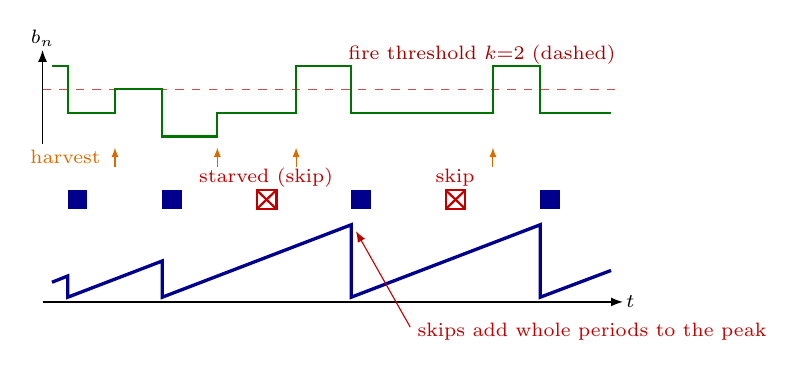
\begin{tikzpicture}[font=\footnotesize,x=1cm,y=1cm]
\colorlet{cbat}{green!45!black}\colorlet{cfire}{blue!55!black}
\colorlet{cskip}{red!75!black}\colorlet{cage}{blue!55!black}
\colorlet{charv}{orange!85!black}
% ===== battery staircase (top band), k=2; levels: b -> 2.1+0.3b =====
\draw[-{Latex[length=1.5mm]}] (-0.12,2.0)--(-0.12,3.2) node[above,font=\scriptsize,inner sep=1pt]{$b_n$};
\draw[dashed,cskip!70] (-0.12,2.7)--(7.25,2.7);
\node[font=\scriptsize,cskip!85!black,anchor=east,inner sep=1pt] at (7.2,3.14) {fire threshold $k{=}2$ (dashed)};
\draw[thick,cbat]
 (0,3.0)--(0.2,3.0)--(0.2,2.4)--(0.8,2.4)--(0.8,2.7)--(1.4,2.7)
 --(1.4,2.1)--(2.1,2.1)--(2.1,2.4)--(3.1,2.4)--(3.1,3.0)--(3.8,3.0)
 --(3.8,2.4)--(5.6,2.4)--(5.6,3.0)--(6.2,3.0)--(6.2,2.4)--(7.1,2.4);
% harvest arrows (below battery band)
\foreach \x in {0.8,2.1,3.1,5.6}{
  \draw[-{Latex[length=1.2mm]},charv] (\x,1.72)--(\x,1.96);}
\node[font=\scriptsize,charv,anchor=east,inner sep=1pt] at (0.66,1.84) {harvest};
% ===== contact comb (middle band): fired (filled) vs starved (crossed) =====
\foreach \x in {0.2,1.4,3.8,6.2}{
  \fill[cfire] (\x,1.18) rectangle (\x+0.25,1.42);}
\foreach \x in {2.6,5.0}{
  \draw[thick,cskip] (\x,1.18) rectangle (\x+0.25,1.42);
  \draw[thick,cskip] (\x,1.18)--(\x+0.25,1.42);
  \draw[thick,cskip] (\x,1.42)--(\x+0.25,1.18);}
\node[font=\scriptsize,align=center,inner sep=1pt,cskip] at (2.72,1.58) {starved (skip)};
\node[font=\scriptsize,align=center,inner sep=1pt,cskip] at (5.12,1.58) {skip};
% ===== age sawtooth (bottom band): resets only at fired windows =====
\draw[-{Latex[length=1.5mm]}] (-0.12,0)--(7.25,0) node[right,font=\scriptsize,inner sep=1pt]{$t$};
\draw[very thick,cage]
 (0,0.25)--(0.2,0.33)--(0.2,0.06)--(1.4,0.52)--(1.4,0.06)
 --(3.8,0.98)--(3.8,0.06)--(6.2,0.98)--(6.2,0.06)--(7.1,0.4);
\draw[-{Latex[length=1.4mm]},cskip] (4.55,-0.32) -- (3.86,0.9);
\node[font=\scriptsize,cskip,anchor=west,inner sep=1pt] at (4.6,-0.38)
  {skips add whole periods to the peak};
\end{tikzpicture}}
\caption{Energy-gated firing, sample path ($k{=}2$). \emph{Top:} the
battery fills by harvest and drops $k$ units at each firing; a window
that opens with $b<k$ is \emph{starved} and skipped (crossed).
\emph{Bottom:} the age resets only at fired windows, so each skip adds a
full period to the peak $JP+R_{\min}+T_s$---the starvation term
$P(1-\peff)/\peff$ of \eqref{eq:obj}. After a firing the battery is
depleted, which is why consecutive windows are correlated
(Markov-renewal gaps) and the fluid throttle is a mean-field limit.}
\label{fig:battpath}
\end{figure}

\begin{lemma}[Work conservation; distribution-free]\label{lem:work}
Each firing slot consumes exactly $k$ units, so in steady state
$k\,\peff(k)=\eta-L$ with $L\ge0$ the mean per-period harvest lost to the
cap. Hence
\begin{equation}
\peff(k)=\frac{\eta-L}{k}\le\min\!\Bigl(1,\frac{\eta}{k}\Bigr),
\end{equation}
with $L=0$ iff no harvested energy is truncated by the cap (the battery
may reach $B$ exactly without loss; only overflowed harvest counts).
\end{lemma}

Only the mean $\eta$ enters at this order; the harvest distribution and
$B$ affect $\peff$ solely through $L$. Thus the throttle of
Section~\ref{sec:r3} is exactly the no-overflow / large-$B$ limit, and
the finite-battery correction is sign-definite ($\peff$ can only be
smaller).

\begin{corollary}[$k=1$ closed form]
Let the per-period harvest increments $A_n$ be i.i.d., nonnegative,
with $\E[A_n]=\eta$ and $\Prob(A_n{=}0)>0$, so the chain
$b_{n+1}=(b_n-1)^+ + A_n$---the
embedded queue-length chain of a discrete-time deterministic-unit-service
queue---is ergodic on the recurrent class reachable from $b_0$ for
$\eta<1$ (all of $\mathbb{N}_0$ under unbounded support, e.g.\
Poisson; trivially for finite $B$); the stated marginals below follow
from flow balance and are class-independent. For $B\to\infty$ and
$\eta<1$, $\Prob_\pi(b=0)=1-\eta$, so $\peff(1)=\eta$, with the
Pollaczek--Khinchine level law. Finite $B$ gives $L\ge0$ and
$\peff(1)\le\eta$, with \emph{strict} loss exactly when overflow has
positive stationary probability---e.g.\ under Poisson harvest for any
finite $B$---but not universally: for Bernoulli harvest
$A_n\in\{0,1\}$ and $B\ge1$ the battery can never overflow, so $L=0$
and $\peff(1)=\eta$ exactly despite the finite cap.
\end{corollary}

\paragraph*{Consequence for $\kstar$}
The objective \eqref{eq:obj} keeps its form---the starvation term
$P(1-\peff)/\peff$ is exact in $\peff$ by the long-run firing
rate---but now with
the true $\peff(k)=(\eta-L(B,k))/k\le\min(1,\eta/k)$. Finite battery thus
weakly enlarges each starvation term, exerting \emph{downward pressure} on
the optimal degree; empirically (E11) $\kstar$
decreases as $B$ shrinks (at $\eta{=}4$: $4\to2$ as $B$ falls
$64\to4$). This is \emph{not} a universal bound
$\kstar\le\lfloor\eta\rfloor$, however: because the overflow loss
$L(B,k)$ depends on $k$, the pointwise bound on $\peff$ does not order
$\mathcal{A}(k)$ across $k$, and a degree that strictly wins in the
infinite-battery limit (e.g.\ $\lceil\eta\rceil$ via \eqref{eq:ceiltest})
still wins for all sufficiently large $B$ (as $B\to\infty$, $L\to0$). The
finite-battery effect is therefore a quantified downward shift, not a hard
ceiling at $\lfloor\eta\rfloor$. In our i.i.d.-harvest scenarios, finite
$B$ also raises the variance of skip gaps (bursty starvation: a firing
depletes the battery, so skips cluster), inflating the PAoI tail but not
the mean; we do not claim this direction universally---under correlated
harvest or other admission policies the gap variance can move either
way, and only the work-conservation identity for the firing
\emph{fraction} is distribution-free.

\paragraph*{Regime-ODE coupling}
Stationary battery--age coupling (steady-state averaging; no
timescale-separation limit is claimed): the battery chain is taken at
its stationary $\pi$ while age evolves under the gated renewal
process. The SHS
mode is $q=(\phi,m)$ with $\phi$ the contact ON/OFF phase and $m$ the
battery regime; the age ODE $\dot\AoI=1$ has delivery resets enabled only
when $m\ge k$, i.e.\ $I^{\mathrm{eff}}(t)=I(t)\,\ind\{b(t)\ge k\}$.
Averaging the gate over the stationary $\pi$ yields the thinned
alternating-renewal schedule of \eqref{eq:thin}: usable windows recur
after $V'=(J{-}1)P+G$ with $\Pr(J{=}j)$ the stationary firing-gap law.
Under i.i.d.\ firing $J$ is geometric and every Result-1 form extends
exactly through the renewal law with $V\to V'$; with a finite battery
the firing gaps are Markov-renewal rather than geometric---after a
firing the battery is depleted, so usable windows cluster---and the
geometric-$J$ forms become a mean-field approximation. Work conservation
(Lemma~\ref{lem:work}) still pins the firing \emph{fraction} at $\peff$
exactly, so the mean starvation term is exact in $\peff$; what the
correlation moves is the firing-gap \emph{variance} (hence the peak-age
tail), which requires the correlated chain. A minimal two-regime
reduction ($m\in\{b<k,\,b\ge k\}$, $\Prob(\text{hi})=\peff$) recovers the
mean; the full $(B{+}1)$-mode generator gives the correlated refinement.

% =====================================================================
\section{An AoI-Energy Replication Policy}\label{sec:policy}
The threshold of Section~\ref{sec:r3} yields a concrete policy that layers
on top of an existing contact-plan router (CGR/RUCoP). CGR computes
\emph{which} routes a bundle can take; the policy decides \emph{how many}
copies to commit, given its long-run energy adequacy. A source that knows its
harvest rate $\lambda_e$, per-copy cost $e$, contact cadence (hence
$\eta=\lambda_e P/e$), and the number $K_{\max}$ of candidate copy
routes CGR offers selects the replication degree by a closed-form
\emph{two-candidate} rule. By \eqref{eq:kstar}--\eqref{eq:ceiltest} the
unconstrained optimum is one of the two integers bracketing $\eta$, so the
policy
evaluates $\mathcal{A}$ at just those two and clips to $[1,K_{\max}]$:
\begin{equation}\label{eq:policy}
\begin{aligned}
k_{\mathrm{pol}}(\eta)&=\arg\min_{k\in\mathcal{K}(\eta)}\mathcal{A}(k),\\
\mathcal{K}(\eta)&=\bigl\{\operatorname{clip}(\lfloor\eta\rfloor,1,K_{\max}),\,
  \operatorname{clip}(\lceil\eta\rceil,1,K_{\max})\bigr\},
\end{aligned}
\end{equation}
with $\mathcal{A}$ from \eqref{eq:obj} (or $\mathcal{A}_q$ from
\eqref{eq:objq} when a route-success estimate is available); it then
commits the $k_{\mathrm{pol}}$ copies and spends only
$k_{\mathrm{pol}}\,e$ per update. The choice is local and $O(1)$ (two
objective evaluations, no sweep over $k$). It is driven by the
\emph{mean} energy-adequacy $\eta$---a slow estimate of harvest rate and
cadence---rather than the instantaneous battery level, and is recomputed
only when that estimate drifts; it is thus a steady-state set-point, not a
per-window controller.

\paragraph*{Joint degree and placement}
\emph{Which} $k_{\mathrm{pol}}$ routes matters as much as how many:
``distinct next-hops'' do not make copy latencies independent---routes
can share source contacts, relays, downstream links, failure domains,
or (per the Iridium scan of Section~\ref{sec:sim}) near-commensurate
orbital phases. Moreover, since replication pays only under route
uncertainty, the placement objective must weigh \emph{timing}
diversity and \emph{failure} diversity together. Both live in one
quantity: for a candidate route set $\mathcal{S}$ with per-route
failure events
$F_i$ (success probability $q_i$, possibly correlated across
routes) and plan-determined residuals $R_i$, the set's success
probability is $s_{\mathcal{S}}=1-\Pr(\bigcap_{i\in\mathcal{S}}F_i)$
and the delivered
residual given success generalizes \eqref{eq:rminjoint} to
\begin{multline}\label{eq:rminsucc}
\E\bigl[R^{\mathrm{succ}}_{\min,\mathcal{S}}\bigr]=\frac{1}{s_{\mathcal{S}}}
\int_0^\infty\Bigl[\Pr\Bigl(\bigcap_{i\in\mathcal{S}}
\bigl(F_i\cup\{R_i>r\}\bigr)\Bigr)\\
-\Pr\Bigl(\bigcap_{i\in\mathcal{S}}F_i\Bigr)\Bigr]dr.
\end{multline}
Under the common periodic firing epoch, single-energy-bottleneck,
constant per-copy-cost model, the exact planning-time problem is the
joint combinatorial one,
\begin{equation}\label{eq:jointopt}
\min_{\varnothing\ne\mathcal{S}\subseteq\mathcal{R},\,
|\mathcal{S}|\le K_{\max}}
\Bigl[\frac{P}{\peff(|\mathcal{S}|)\,s_{\mathcal{S}}}
+\E\bigl[R^{\mathrm{succ}}_{\min,\mathcal{S}}\bigr]\Bigr],
\end{equation}
in which the best set can change the best \emph{degree} (a pair with
poor common-mode reliability can lose to a three-route set with better
failure-domain diversity); for heterogeneous routes---distinct periods,
route-dependent energy, route-specific launch epochs---the cadence term
$P/(\peff s_{\mathcal{S}})$ is replaced by the set's actual mean
inter-successful-update interval. We do not solve \eqref{eq:jointopt}
here.
The precise reading of our components is: \eqref{eq:policy} is the
$O(1)$ degree set-point that is exact for a statistically
\emph{exchangeable} route pool (i.i.d.\ successes, ensemble phases,
where \eqref{eq:jointopt} reduces to \eqref{eq:objq}); the
\eqref{eq:rminsucc}-based set choice at fixed $|\mathcal{S}|$ is a
placement \emph{refinement}; and fully joint heterogeneous
degree-and-placement optimization is an extension. Note the $O(1)$
claim covers the degree rule only---evaluating \eqref{eq:rminsucc}
over route subsets is combinatorial, with disjointness and
pairwise-correlation proxies as the cheap surrogates. The two
diversities can trade off: an
anti-phased pair sharing a failure domain (correlated $F_i$, small
$s_{\mathcal{S}}$) can lose to a slightly less anti-phased pair with
independent
failures---timing diversity optimizes
$\E[R^{\mathrm{succ}}_{\min}]$,
failure diversity optimizes $s_{\mathcal{S}}$, and \eqref{eq:rminsucc}
prices both.
On the real constellation the timing axis alone already spans more
than the degree step: the best-aligned Iridium pair reaches a
residual-min ratio of
$0.41$ where a blind pick averages ${\sim}0.65$ and a phase-locked pair
returns $0.95$.

We evaluate the policy in the finite-battery model against every fixed
degree $k=1,\dots,K_{\max}$ and against the per-$\eta$ exhaustive optimum
(Fig.~\ref{fig:policy}). The closed-form rule \eqref{eq:policy} matched
the exhaustive optimum at all sampled energy levels, and its PAoI is the
lower envelope of the fixed-degree curves: any fixed $k$ is wasteful when
energy is scarce (a large $k$ starves) or stale when it is abundant (a
small $k$ forgoes the order-statistic gain), whereas the adaptive policy
is best at every energy level. We stress the scope of this statement:
the two-candidate rule is derived in the large-battery model, and there
is \emph{no theorem} that the finite-battery optimum stays in
$\{\lfloor\eta\rfloor,\lceil\eta\rceil\}$ in general---it did so in
every tested $(\eta,B)$ configuration, but our own E15 experiment
exhibits the boundary: under strongly persistent (dwell${\approx}50$)
Markov-modulated harvest the optimum moves to $k{=}2<\lfloor\eta\rfloor$
at $\eta{=}3$, outside the candidate set. The policy is thus an
empirically robust set-point with a measured failure regime, not a
finite-battery optimality theorem. It is realized in a DTN-realistic
stack by our CGR-native $k$-copy router (Section~\ref{sec:sim}).

\paragraph*{Worked example (Iridium-class numbers)}
Take the paper's LEO scenario: $P=5736$\,s, $W=430$\,s
($\delta=0.075$), $T_s=10$\,s, and a solar harvest that accumulates one
copy's energy every $2200$\,s, so $\eta=\lambda_e P/e=2.6$. The two
candidates are $k\in\{2,3\}$; the ceiling test \eqref{eq:ceiltest}
compares added starvation $P(3/2.6-1)=882$\,s against order-statistic
gain $g_2-g_3=463$\,s, so the floor wins: $k_{\mathrm{pol}}=2$. The
resulting mean $\PAoIper$ is $P+\E[R_{\min,2}]+T_s=5736+1513+10\approx
7.3\times10^3$\,s ($\approx 2.0$\,h), versus $8.2\times10^3$\,s
($\approx2.3$\,h) single-copy---a $12\%$ freshness gain for one extra
copy---whereas $k{=}3$ would \emph{lose} ground
($\mathcal{A}(3)-\mathcal{A}(2)\approx+419$\,s) by starving one window in
$7.5$.

\paragraph*{Tail / deadline-violation}
For mission-critical traffic the relevant quantity is the PAoI
\emph{tail}, $\Pr(\PAoIper>\Delta)$, not the mean---and in the LEO $k$-copy
model the tail is available in closed form.

\begin{corollary}[$\PAoIper$ tail, LEO $k$-copy]\label{cor:tail}
Under the model of Section~\ref{sec:r3} with i.i.d.\ firing (exact when
$\peff=1$; mean-field otherwise), the per-update peak decomposes as
$\PAoIper=JP+R_{\min,k}+T_s$ with $J\sim\mathrm{Geom}(\peff)$ independent of
$R_{\min,k}$. For $x=T_s+jP+r$, $j\ge1$, $r\in[0,P)$,
\begin{multline}\label{eq:tailcf}
\Pr(\PAoIper>x)=(1-\peff)^{j}\\
+\peff(1-\peff)^{j-1}\Bigl(\tfrac{G-r}{P}\Bigr)^{k}\ind\{r\le G\},
\end{multline}
and in the energy-abundant regime ($\peff{=}1$) the $\beta$-quantile is
$T_s+P+\max\bigl\{0,\;G-P(1-\beta)^{1/k}\bigr\}$: the maximum handles the
atom of $R_{\min,k}$ at $0$ (mass $1-(G/P)^k$, an update generated
inside a window), at which the quantile sits for all
$q\le1-(G/P)^k$.
\end{corollary}

Replication thus pulls the tail in polynomially---degree $k$ in the gap
fill---and the simulated CCDF (Fig.~\ref{fig:ccdf}) matches
\eqref{eq:tailcf} pointwise: at a $1.5P$ deadline the closed form gives
$0.405^{k}$ $=0.405,\,0.164,\,0.027$ for $k{=}1,2,4$ against simulated
$0.405,\,0.165,\,0.027$ (a $15\times$ reduction at $k{=}4$), and the
$99$th percentile $T_s+P+G-P(0.01)^{1/k}$ evaluates to $1.90P$ ($k{=}1$)
and $1.59P$ ($k{=}4$), exactly the simulated quantiles. For a renewal
segment the single-copy tail is immediate from \eqref{eq:renewal}:
$\Pr(\OPAoI>x)=\Pr(V>x-T_s)$. The mean alone therefore understates the
value of replication; the policy \eqref{eq:policy} extends to a deadline
constraint by minimizing $\mathcal{A}$ subject to
$\Pr(\PAoIper>\Delta)\le\epsilon$ with the left side evaluated by
\eqref{eq:tailcf} rather than simulation.

\paragraph*{Comparison with a RUCoP-style MDP core}
RUCoP/CGR-UCoP casts routing under \emph{uncertain} contact plans as an
MDP that maximizes delivery probability for a copy budget. Rather than
reproduce the full CGR-UCoP pipeline, we implemented its decision core---a
RUCoP-style holder-set backward induction over the time-ordered contacts,
budgeting transmissions and validated against the closed form $1-(1-q)^k$
on a symmetric plan---and solved it on a single heterogeneous uncertain
diamond to obtain a delivery-vs-copies frontier (an illustrative
instance, not a benchmark-scale reproduction). The two approaches are
complementary: the MDP answers \emph{which} routes maximize delivery and
is energy-blind---its optimum operates at the budget ceiling
$k{=}K_{\max}$---whereas our policy answers \emph{how many} copies the
energy budget warrants. On this instance the frontier is concave, so
copies beyond the knee buy little delivery: at $k^\ast{=}2$ our policy
attains $94.7\%$ of the MDP's delivery for $40\%$ of the energy (the exact
percentages are instance-specific; the concavity, not the number, is the
point). The two compose---the MDP's route set under our degree cap---which
is the natural energy-aware extension of CGR-UCoP.

\paragraph*{Robustness to contact-prediction error}
Contact plans are predictions. We model a prediction reliability
$\alpha$: each committed copy's predicted contact materializes w.p.\
$\alpha$, with energy spent on the commit regardless (a copy sent to a
missed contact is wasted). A natural intuition is to reserve energy under
uncertainty---use $\lfloor\alpha\eta\rfloor$ copies. Our experiments show
the opposite: the PAoI-optimal degree stays at the
no-starvation degree $\lfloor\eta\rfloor$ for every $\alpha\in[0.4,1]$
(here $\eta$ is set so $\lfloor\eta\rfloor$ is the model optimum), because
extra copies hedge missed contacts through the order statistic over which
copies materialize. The rule therefore degrades gracefully ($+19\%$ PAoI
as $\alpha$ falls to $0.4$), whereas the reserve heuristic
under-replicates and is counterproductive ($+50\%$ PAoI at $\alpha{=}0.4$).
In the tested regime---independent per-copy materialization with energy
spent regardless---replication, not a smaller copy budget, is the right
response to prediction uncertainty; this is now also a \emph{prediction}
of Proposition~\ref{prop:uncertain} with $q{=}\alpha$ rather than only
an observation. With correlated failures, asymmetric route
probabilities, or route-dependent energy costs the optimal response can
differ, and the $q$-model would need the corresponding generalization.

% =====================================================================
\section{Numerical Validation}\label{sec:sim}
Validation follows a two-tier plan, closed by a reference-implementation
cross-check. A model-exact Monte-Carlo simulator
confirms the closed forms over the parameter sweeps (duty cycle $\delta$,
replication degree $k$, energy-adequacy $\eta$, battery capacity $B$); a
DTN-realistic stack with Bundle Protocol and Contact Graph Routing
(\texttt{dtnsim}, the contact-plan simulator of the RUCoP/CGR-UCoP
lineage), extended with a custom energy-harvesting battery module and a
CGR-native $k$-copy router, runs the representative scenarios and compares
single-copy CGR against CGR replication under an energy budget. A RUCoP-style MDP core is implemented and compared on an illustrative
instance in Section~\ref{sec:policy}.
Each theoretical claim maps to one experiment with a quantitative pass
criterion: the mixed residual law and the quadratic-mean/linear-peak
divergence of Theorem~\ref{thm:r1}; the fixed-plan mixing approximation and its phase-locking failure
mode (Remark~\ref{rem:fixedmix}); the Gini-dispersion replication
gain and its collapse for same-bottleneck copies (Theorem~\ref{thm:r2});
the unimodal objective and threshold $\kstar$ with monotonicity and
saturation (Theorem~\ref{thm:r3}); and the work-conservation throttle
with the finite-battery correction and its downward pressure on $\kstar$
(Lemma~\ref{lem:work}). Scenario specifications and contact plans are
released for reproducibility.

\paragraph*{Tier-1 results}
Table~\ref{tab:tier1} traces every analytical claim to its model-exact
experiment (time normalized to $P{=}1$; $8$--$20$ seeded replications
with 95\% CIs); all pass. Two rows warrant prose. The \emph{ceiling}
branch flips exactly at the analytic crossover of \eqref{eq:ceiltest}
($\delta{=}0.1$ on $[3,4]$: simulated flip between $\eta{=}3.8$ and
$3.9$, $\eta^\star{=}3.824$), so the extra copy is taken precisely when
its gain repays the added starvation. And the bursty-harvest row is the
policy's measured \emph{failure boundary}: the threshold and the
work-conservation identity survive Markov-modulated harvest up to a
mean dwell of ten periods (correlation moves the tail, $1.78P\to3.07P$
at $\kstar$---the Markov-renewal effect anticipated in
Section~\ref{sec:r3hard}), but under extreme persistence (dwell
${\approx}50$) the optimum retreats to $k{=}2$, the regime where a
mean-based set-point should yield to regime-aware adaptation
(cf.\ Section~\ref{sec:policy}).

\begin{table}[t]
\caption{Tier-1 traceability: analytical claim $\to$ model-exact check.}
\label{tab:tier1}
\centering
\renewcommand{\arraystretch}{1.18}
\setlength{\tabcolsep}{3pt}
\footnotesize
\begin{tabular}{>{\raggedright\arraybackslash}p{0.24\columnwidth}>{\raggedright\arraybackslash}p{0.315\columnwidth}>{\raggedright\arraybackslash}p{0.315\columnwidth}}
\hline
Claim & Check & Outcome \\
\hline
Residual law, Thm~\ref{thm:r1} & KS to mixed law; mean/peak exponents in $(1{-}\delta)$ & KS $0.002$; slopes $1.98/1.00$ (Fig.~\ref{fig:r1}) \\
Fixed-plan mixing, Rem.~\ref{rem:fixedmix} & phase KS-to-uniform, corr.; commensurate control & $0.001$, $|\rho|{=}0.002$; locked: KS $0.89$ \\
Two-copy gain, Thm~\ref{thm:r2} & Gini identity; ratio $\tfrac23(1{-}\delta)$; same-bottleneck & matched (Fig.~\ref{fig:r2gain}); zero gain \\
Threshold, \eqref{eq:kstar}, Thm~\ref{thm:r3} & unimodality; staircase, saturation & argmin brackets $\eta$ (Figs.~\ref{fig:r3unimodal},~\ref{fig:r3kstar}) \\
Ceiling branch \eqref{eq:ceiltest} & fine $\eta$-sweep on $[3,4]$ & flip at $\eta^\star{=}3.824$ \\
Work cons., Lem.~\ref{lem:work} & $k\peff{=}\eta{-}L$; $k{=}1$ P--K law; Poisson vs.\ deterministic & $\le\!10^{-5}$; distribution-free; $\peff(1){=}\eta$ \\
Finite $B$, Sec.~\ref{sec:r3hard} & $\kstar$ vs.\ $B$ (E11) & $4\to2$ as $B$: $64\to4$ ($\eta{=}4$) \\
Bursty harvest & Markov-modulated dwell sweep, $\eta{=}3$ & $\kstar$ invariant to dwell $10$; wc $\le\!3{\times}10^{-4}$; $k{=}2$ at dwell $50$ \\
Renewal laws \eqref{eq:renewal},\newline\eqref{eq:invcond} & det., jitter, exp., Pareto; inversion threshold & $\E[R]$ within $1\%$; crossing matched (Fig.~\ref{fig:inversion}) \\
Uncertainty, Prop.~\ref{prop:uncertain} & \eqref{eq:objq} vs.\ sim over $q{\times}k{\times}\eta$ & within $0.7\%$; optimum in candidate set \\
\hline
\end{tabular}
\end{table}

% AUTO-GENERATED by figs/make_figures.py from sim/results/*.csv
% and sim/tier2/results/*.csv. Re-run the generator to refresh.
% Colour palette: Okabe-Ito (colour-blind safe, prints legibly in grey).
\definecolor{cA}{RGB}{0,114,178}
\definecolor{cB}{RGB}{213,94,0}
\definecolor{cC}{RGB}{0,158,115}
\definecolor{cD}{RGB}{204,121,167}
\definecolor{cE}{RGB}{230,159,0}
\pgfplotsset{
  paperfig/.style={
    grid=both, grid style={black!10},
    legend cell align=left,
    legend style={font=\scriptsize, fill=white, fill opacity=0.92,
                  text opacity=1, draw=black!45, inner xsep=3pt,
                  inner ysep=1.6pt, rounded corners=1pt},
    tick label style={font=\footnotesize},
    label style={font=\footnotesize},
  }
}

\begin{figure}[t]\centering
\begin{tikzpicture}
\begin{axis}[paperfig,width=\columnwidth,height=0.66\columnwidth,
  xlabel={duty cycle $\delta$},ylabel={age (normalized, $P{=}1$)},
  legend style={at={(0.5,-0.26)},anchor=north,legend columns=2},
  error bars/y dir=both,error bars/y explicit]
\addplot[cA,only marks,mark=*,mark size=1.5pt] coordinates {(0.02,0.9870100715269062) +- (0,3.1292142984718735e-05) (0.05,0.9569975439410504) +- (0,2.8138476284065702e-05) (0.075,0.9320010411719328) +- (0,2.902494335842732e-05) (0.1,0.9069955973162998) +- (0,1.893193054617168e-05) (0.2,0.8069971556041535) +- (0,2.4082530275375084e-05) (0.35,0.657020357263457) +- (0,2.364619973598577e-05) (0.5,0.5069971053296146) +- (0,2.473059005205108e-05)};
\addlegendentry{OPAoI (sim)}
\addplot[cA,no marks,thick,dashed] coordinates {(0.02,0.985) (0.05,0.955) (0.075,0.93) (0.1,0.905) (0.2,0.805) (0.35,0.655) (0.5,0.505)};
\addlegendentry{OPAoI $=T_s+P(1-\delta)$}
\addplot[cB,only marks,mark=square*,mark size=1.5pt] coordinates {(0.02,0.48721054412512643) +- (0,3.05966842493133e-05) (0.05,0.45824685360113504) +- (0,2.693793306118609e-05) (0.075,0.4348135198357405) +- (0,2.655059400816846e-05) (0.1,0.4119961987610867) +- (0,1.6638518202369598e-05) (0.2,0.3269977862109709) +- (0,1.944432796664332e-05) (0.35,0.21826373712641028) +- (0,1.6032026469115834e-05) (0.5,0.13199933546467407) +- (0,1.2466013684464939e-05)};
\addlegendentry{mean AoI (sim)}
\addplot[cB,no marks,thick,densely dotted] coordinates {(0.02,0.48519999999999996) (0.05,0.45625) (0.075,0.43281250000000004) (0.1,0.41000000000000003) (0.2,0.32500000000000007) (0.35,0.21625000000000003) (0.5,0.13)};
\addlegendentry{mean AoI $=T_s+\tfrac{P}{2}(1-\delta)^2$}
\end{axis}
\end{tikzpicture}
\caption{Result~1 (E1/E2): simulated mean AoI and OPAoI vs.\ duty cycle
match the closed forms; the peak grows linearly and the mean
quadratically in $(1-\delta)$ (provisioning divergence). Markers are
Monte-Carlo means with 95\% CIs (smaller than markers).}
\label{fig:r1}
\end{figure}


\begin{figure}[t]\centering
\begin{tikzpicture}
\begin{axis}[paperfig,width=\columnwidth,height=0.6\columnwidth,
  xlabel={duty cycle $\delta$},ylabel={$\mathbb{E}[R_{\min}]/\mathbb{E}[R]$},
  legend pos=north east,grid=both,legend cell align=left]
\addplot[cA,only marks,mark=*,mark size=1.6pt] coordinates {(0.02,0.653362323347421) (0.05,0.6333883269504517) (0.1,0.6001979804547108) (0.2,0.5336253055696409) (0.35,0.433159970801058) (0.5,0.33323957490210027)};
\addlegendentry{sim}
\addplot[cB,no marks,thick,dashed] coordinates {(0.02,0.6533333333333333) (0.05,0.6333333333333333) (0.1,0.6) (0.2,0.5333333333333333) (0.35,0.43333333333333335) (0.5,0.3333333333333333)};
\addlegendentry{$\tfrac{2}{3}(1-\delta)$}
\end{axis}
\end{tikzpicture}
\caption{Result~2 (E4): the two-copy gain. Simulated
$\mathbb{E}[R_{\min}]/\mathbb{E}[R]$ matches the two-copy
ratio $\tfrac{2}{3}(1-\delta)$; replication saves most at sparse
contacts ($\delta\to0$).}
\label{fig:r2gain}
\end{figure}


\begin{figure}[t]\centering
\begin{tikzpicture}
\begin{axis}[paperfig,width=\columnwidth,height=0.66\columnwidth,
  xlabel={replication degree $k$},ylabel={mean $\PAoIper$ (normalized)},
  legend pos=north west,grid=both,legend cell align=left,xtick=data]
\addplot[thick,cA,mark=*,mark size=1.3pt] coordinates {(1.0,1.410314663389778) (2.0,1.248192570863487) (3.0,1.1777586195908003) (4.0,1.4564704134531814) (5.0,1.7592147238268279) (6.0,2.073176697683509) (7.0,2.3922001335971532) (8.0,2.7185592470423137) (9.0,3.0510884750494167)};
\addlegendentry{$\eta=3$ ($k^\ast=3$)}
\addplot[thick,cB,mark=square*,mark size=1.3pt] coordinates {(1.0,1.4101859347850572) (2.0,1.2478719880669222) (3.0,1.1692371885105677) (4.0,1.123112635056019) (5.0,1.1020916179657483) (6.0,1.2732102430111434) (7.0,1.458191515479616) (8.0,1.6476294592829408) (9.0,1.8487261126269243)};
\addlegendentry{$\eta=5$ ($k^\ast=5$)}
\end{axis}
\end{tikzpicture}
\caption{Result~3 (E7): the integrated energy+replication+AoI objective
is unimodal in $k$ with minimum at one of the two integers bracketing
$\eta$; pushing
$k$ past the energy budget starves future contacts and raises the peak.}
\label{fig:r3unimodal}
\end{figure}


\begin{figure}[t]\centering
\begin{tikzpicture}
\begin{axis}[paperfig,width=\columnwidth,height=0.6\columnwidth,
  xlabel={energy-adequacy ratio $\eta=\lambda_e P/e$},ylabel={optimal degree $k^\ast$},
  legend pos=south east,grid=both,legend cell align=left,ymin=0]
\addplot[cB,no marks,thick,dashed,const plot] coordinates {(1.0,1.0) (2.0,2.0) (3.0,3.0) (4.0,4.0) (6.0,6.0) (8.0,8.0) (10.0,8.0)};
\addlegendentry{$\min(K_{\max},\lfloor\eta\rfloor)$}
\addplot[cA,only marks,mark=*,mark size=1.7pt] coordinates {(1.0,1.0) (2.0,2.0) (3.0,3.0) (4.0,4.0) (6.0,6.0) (8.0,8.0) (10.0,8.0)};
\addlegendentry{sim}
\end{axis}
\end{tikzpicture}
\caption{Result~3 (E8): $k^\ast(\eta)$ is non-decreasing in the
harvest-to-contact ratio and saturates at $K_{\max}{=}8$ once energy
ceases to bind.}
\label{fig:r3kstar}
\end{figure}


\begin{figure}[t]\centering
\begin{tikzpicture}
\begin{axis}[paperfig,width=\columnwidth,height=0.6\columnwidth,
  xlabel={gap coefficient of variation $\mathrm{CV}(V)$},
  ylabel={age (normalized)},legend pos=north west,grid=both,
  legend cell align=left]
\addplot[cB,only marks,mark=square*,mark size=1.7pt] coordinates {(0.0,0.41) (0.3,0.44625348238863416) (0.5,0.5108772600771613) (1.0,0.8149996897795648) (1.5,1.3224004704089134) (2.0,2.030147837685105)};
\addlegendentry{mean AoI}
\addplot[cA,only marks,mark=*,mark size=1.7pt] coordinates {(0.0,0.9049999999999999) (0.3,0.9046423617422175) (0.5,0.9044223082534586) (1.0,0.9043348492407165) (1.5,0.9039569330472569) (2.0,0.9033825094312596)};
\addlegendentry{mean OPAoI}
\draw[gray,dashed] (axis cs:1.106,\pgfkeysvalueof{/pgfplots/ymin}) -- (axis cs:1.106,\pgfkeysvalueof{/pgfplots/ymax});
\end{axis}
\end{tikzpicture}
\caption{The AoI/OPAoI inversion (E12). Mean OPAoI ($=T_s+
\mathbb{E}[V]$) is flat in the gap variability, while mean AoI grows
with it; they cross at the exact threshold
$\mathrm{CV}^2(V)=1+2\mathbb{E}[U]/\mathbb{E}[V]$ (dashed:
$\mathrm{CV}\approx1.11$ for the plotted $\mathbb{E}[U]/\mathbb{E}[V]=1/9$),
so for high-variance
terrestrial contacts the outage peak sits {\itshape below}
average AoI.}
\label{fig:inversion}
\end{figure}


\begin{figure}[t]\centering
\begin{tikzpicture}
\begin{axis}[paperfig,width=\columnwidth,height=0.62\columnwidth,
  xlabel={energy-adequacy ratio $\eta$},ylabel={mean PAoI (normalized)},
  legend pos=north east,grid=both,legend cell align=left,ymax=4.2]
\addplot[cC,semithick,densely dotted,mark=triangle*,mark size=1.5pt] coordinates {(0.5,2.406) (1.0,1.418) (1.5,1.410) (2.0,1.410) (2.5,1.410) (3.0,1.410) (3.5,1.410) (4.0,1.410) (5.0,1.410) (6.0,1.410) (8.0,1.411)};
\addlegendentry{fixed $k{=}1$}
\addplot[cE,semithick,dashdotted,mark=square*,mark size=1.5pt] coordinates {(0.5,4.244) (1.0,2.246) (1.5,1.580) (2.0,1.256) (2.5,1.248) (3.0,1.248) (3.5,1.248) (4.0,1.248) (5.0,1.248) (6.0,1.248) (8.0,1.248)};
\addlegendentry{fixed $k{=}2$}
\addplot[cD,semithick,densely dashed,mark=diamond*,mark size=1.6pt] coordinates {(0.5,8.111) (1.0,4.121) (1.5,2.787) (2.0,2.122) (2.5,1.723) (3.0,1.455) (3.5,1.265) (4.0,1.131) (5.0,1.123) (6.0,1.123) (8.0,1.123)};
\addlegendentry{fixed $k{=}4$}
\addplot[cA,very thick,mark=*,mark size=1.8pt] coordinates {(0.5,2.406) (1.0,1.418) (1.5,1.410) (2.0,1.256) (2.5,1.248) (3.0,1.177) (3.5,1.169) (4.0,1.131) (5.0,1.123) (6.0,1.123) (8.0,1.123)};
\addlegendentry{AoI-Energy policy}
\end{axis}
\end{tikzpicture}
\caption{The AoI-Energy policy selects the replication degree from the
closed-form rule $k_{\mathrm{pol}}(\eta)=\arg\min_k\mathcal{A}(k)$
(no search); it matched the per-$\eta$ exhaustive optimum in all 11 cases
and is the lower envelope of every fixed-degree curve. A single fixed $k$
is wasteful when energy is scarce (large $k$ starves) or stale when it is
abundant (small $k$ misses the order-statistic gain); the adaptive policy
is best at every energy level.}
\label{fig:policy}
\end{figure}


\begin{figure}[t]\centering
\begin{tikzpicture}
\begin{semilogyaxis}[paperfig,width=\columnwidth,height=0.6\columnwidth,
  xlabel={deadline $\Delta$ (periods $P$)},
  ylabel={$\Pr(\PAoIper>\Delta)$},legend pos=south west,grid=both,
  legend cell align=left,ymin=0.0008,ymax=1.2]
\addplot[cC,thick,densely dotted,mark=triangle*,mark size=1.5pt] coordinates {(1.0,1.00000) (1.05,0.85442) (1.1,0.80444) (1.15,0.75449) (1.2,0.70461) (1.25,0.65425) (1.3,0.60426) (1.35,0.55411) (1.4,0.50408) (1.45,0.45433) (1.5,0.40460) (1.55,0.35457) (1.6,0.30521) (1.65,0.25518) (1.7,0.20550) (1.75,0.15537) (1.8,0.10531) (1.85,0.05534) (1.9,0.00499) (1.95,0.00010) (2.0,0.00010)};
\addlegendentry{$k{=}1$}
\addplot[cE,thick,dashed,mark=square*,mark size=1.5pt] coordinates {(1.0,1.00000) (1.05,0.73057) (1.1,0.64790) (1.15,0.56975) (1.2,0.49702) (1.25,0.42933) (1.3,0.36668) (1.35,0.30882) (1.4,0.25571) (1.45,0.20794) (1.5,0.16468) (1.55,0.12647) (1.6,0.09356) (1.65,0.06516) (1.7,0.04208) (1.75,0.02393) (1.8,0.01093) (1.85,0.00297) (1.9,0.00010) (1.95,0.00010) (2.0,0.00010)};
\addlegendentry{$k{=}2$}
\addplot[cA,thick,mark=*,mark size=1.5pt] coordinates {(1.0,1.00000) (1.05,0.53382) (1.1,0.41980) (1.15,0.32479) (1.2,0.24730) (1.25,0.18397) (1.3,0.13372) (1.35,0.09478) (1.4,0.06520) (1.45,0.04305) (1.5,0.02712) (1.55,0.01604) (1.6,0.00868) (1.65,0.00418) (1.7,0.00172) (1.75,0.00054) (1.8,0.00011) (1.85,0.00010) (1.9,0.00010) (1.95,0.00010) (2.0,0.00010)};
\addlegendentry{$k{=}4$}
\end{semilogyaxis}
\end{tikzpicture}
\caption{PAoI tail (deadline-violation probability) at energy-abundant
$\eta$: replication pulls in the tail via the order statistic. The
probability of exceeding a $1.5P$ freshness deadline falls from $0.40$
($k{=}1$) to $0.16$ ($k{=}2$) to $0.027$ ($k{=}4$)---a $15\times$
reduction---and the $99$th-percentile PAoI drops from $1.90P$ to $1.59P$.
Mean PAoI alone understates the benefit of replication for
mission-critical traffic.}
\label{fig:ccdf}
\end{figure}


\begin{figure}[t]\centering
\begin{tikzpicture}
\begin{axis}[paperfig,width=\columnwidth,height=0.6\columnwidth,
  xlabel={energy-adequacy ratio $\eta$ (harvest per update $/\,e$)},
  ylabel={mean OPAoI (periods $P$)},
  legend style={at={(0.97,0.52)},anchor=east},
  error bars/y dir=both,error bars/y explicit]
\addplot[cB,thick,mark=square*,mark size=1.6pt] coordinates {(0.6,8.886) +- (0,0.110) (0.99,8.810) +- (0,0.116) (1.5,8.635) +- (0,0.166) (2.01,8.527) +- (0,0.108) (3.0,8.102) +- (0,0.303) (6.0,7.006) +- (0,0.575)};
\addlegendentry{single-copy CGR}
\addplot[cA,thick,mark=*,mark size=1.6pt] coordinates {(0.6,1.393) +- (0,0.034) (0.99,1.361) +- (0,0.022) (1.5,1.334) +- (0,0.038) (2.01,1.320) +- (0,0.030) (3.0,1.249) +- (0,0.020) (6.0,1.193) +- (0,0.037)};
\addlegendentry{CGR $k{=}2$ (this work)}
\end{axis}
\end{tikzpicture}
\caption{Replication benefit in a real CGR stack with our CGR-native
$k$-copy router (dtnsim, random relay faults, source energy gate; 10
seeds, 95\% CIs). Sending two copies over the two best distinct CGR
routes cuts mean OPAoI by roughly $6\times$ versus single-copy across the
whole energy range---the order statistic hedges relay faults. Because the
per-transmission energy gate defers the second copy when the battery is
low (rather than dropping the update), the benefit degrades gracefully as
$\eta$ falls instead of inverting. This experiment isolates the
fault-hedging \emph{mechanism}; it is not a test of the atomic
all-or-nothing policy of \eqref{eq:kstar}, whose over-replication
penalty appears in Fig.~\ref{fig:r3atomic}.}
\label{fig:r3tier2}
\end{figure}


\begin{figure}[t]\centering
\begin{tikzpicture}
\begin{axis}[paperfig,width=\columnwidth,height=0.62\columnwidth,
  xlabel={replication degree $k$ (atomic all-or-nothing admission)},
  ylabel={mean OPAoI (periods $P$)},legend pos=north west,grid=both,
  legend cell align=left,xtick={1,2,3}]
\addplot[thick,cA,mark=*,mark size=1.6pt] coordinates {(1,1.760) (2,3.432) (3,5.101)};
\addlegendentry{$\eta=0.6$}
\addplot[thick,cB,mark=square*,mark size=1.6pt] coordinates {(1,1.162) (2,2.096) (3,3.096)};
\addlegendentry{$\eta=1$}
\addplot[thick,cD,mark=diamond*,mark size=1.6pt] coordinates {(1,1.162) (2,1.162) (3,1.598)};
\addlegendentry{$\eta=2$}
\addplot[thick,cE,mark=pentagon*,mark size=1.6pt] coordinates {(1,1.162) (2,1.162) (3,1.162)};
\addlegendentry{$\eta=3$}
\end{axis}
\end{tikzpicture}
\caption{Tier-2 atomic threshold test (real CGR, fault-free
3-relay staggered diamond, update-atomic admission: launch $k$ copies
iff the battery holds $k$ units, else skip the whole update; 5 seeds).
The over-replication penalty is now visible in the DTN stack:
at $\eta{=}1$, $k{=}3$ admits $35\%$ of updates (theory
$\min(1,\eta G_{\mathrm{gen}}/kP)$, matched to $<0.5\%$) and its
peak age is $2.7\times$ single-copy's. At $\eta\ge3$ the degrees tie
exactly: with a fault-free deterministic plan, oracle CGR's single copy
already rides the earliest route, so extra copies deliver stale
duplicates---the strict replication benefit requires route-outcome
uncertainty (Fig.~\ref{fig:r3tier2}).}
\label{fig:r3atomic}
\end{figure}


\begin{figure}[t]\centering
\begin{tikzpicture}
\begin{axis}[paperfig,width=\columnwidth,height=0.6\columnwidth,
  xlabel={relay battery capacity $B$ (copies)},
  ylabel={end-to-end mean OPAoI (periods $P$)},grid=both,
  xmode=log,log basis x=2,legend pos=north east,legend cell align=left]
\addplot[cA,thick,mark=*,mark size=1.5pt] coordinates {(4.0,19.361) (8.0,14.100) (16.0,2.487) (32.0,1.844) (64.0,1.802)};
\addlegendentry{heterogeneous chain}
\addplot[cC,thick,dashed,no marks] coordinates {(4,1.802) (64,1.802)};
\addlegendentry{energy-unconstrained}
\end{axis}
\end{tikzpicture}
\caption{Energy coupling in the full heterogeneous chain (sensor $\to$ UAV
mule $\to$ LEO $\to$ gateway in real CGR). A finite battery at the UAV/LEO
relays must cover the per-contact forwarding burst; below that, end-to-end
mean OPAoI degrades by $\sim\!11\times$ (and delivery collapses from $96\%$
to $31\%$). With sufficient battery it matches the energy-unconstrained
chain, whose mean delay confirms the additive composition
$\E[Y]{=}\E[R_1]{+}\E[R_2]{+}\E[R_3]$ to $1.1\%$.}
\label{fig:hetero}
\end{figure}


\paragraph*{Tier-2 results (DTN-realistic CGR)}
We reproduce the findings in dtnsim, a Bundle-Protocol/Contact-Graph-
Routing simulator of the CGR lineage, over the same scenarios with a
custom energy-harvesting battery module. Result~1: routing periodic
status updates over a real contact plan yields a mean delivery delay of
$2453.9$\,s against the closed-form $\E[R]{=}2453.9$\,s, and the
delay histogram reproduces the full mixed residual law (atom plus uniform
slab). Result~2: for a two-segment relay, the end-to-end latency standard
deviation matches $\sqrt{\operatorname{Var}R_1+\operatorname{Var}R_2}$
under incommensurate segment periods (independence) but collapses toward
$\sqrt{\operatorname{Var}R_1}$ under commensurate periods (phase locking),
supporting the fixed-plan mixing approximation of
Remark~\ref{rem:fixedmix} and demonstrating its phase-locking failure
mode (Lemma~\ref{lem:mix} remains the exact random-offset
result). The renewal residual
law \eqref{eq:renewal} holds within $0.5\%$ across contact-gap laws
(gamma, and genuinely heavy-tailed Pareto), and the AoI/PAoI inversion
(Remark~\ref{rem:inversion}) appears once
$\mathrm{CV}^2(V)>1+2\E[U]/\E[V]$ per \eqref{eq:invcond}. Result~3: we implemented a CGR-native $k$-copy router that commits a copy
to each of the $k$ best distinct CGR routes (approximating independence), and compared it against
single-copy CGR under random relay faults and a source energy gate.
Scenario: the three-relay diamond of Fig.~\ref{fig:r3tier2}; each relay
fails and recovers independently with exponential time-to-failure and
time-to-repair of mean $8000$\,s and $4000$\,s respectively (each
relay is down $1/3$ of the time); the source battery gates each copy at cost $e$ with the
harvest-rate sweep setting $\eta$; $10$ fault/harvest seeds, $95\%$
CIs; full scenario files ship with the artifact. Two copies cut mean $\OPAoI$ by roughly $6\times$
across the entire energy range (Fig.~\ref{fig:r3tier2}; e.g.\ $7.0P$
single-copy versus $1.2P$ with two copies at $\eta{=}6$, with
non-overlapping CIs)---the order
statistic over two relay-disjoint CGR routes with independent
relay-fault processes hedges relay faults. Because the
per-transmission energy gate defers the second copy when the battery is
low rather than dropping the update, the benefit \emph{degrades
gracefully} as $\eta$ falls instead of inverting. The threshold's
\emph{starvation} side is then validated in the DTN stack directly with
\emph{update-atomic} all-or-nothing admission (launch $k$ copies iff
the battery holds $k$ units, else skip the whole update) on a
fault-free three-relay staggered diamond
(Fig.~\ref{fig:r3atomic}): admitted fractions match
$\min(1,\eta G_{\mathrm{gen}}/kP)$ to $<0.5\%$ at every $(\eta,k)$, and
over-replication is punished exactly as \eqref{eq:obj} predicts---at
$\eta{=}1$, $k{=}3$ skips two of three updates and its peak age is
$2.7\times$ single-copy's. The same experiment measures
Remark~\ref{rem:uncertainty} in real CGR: fault-free, higher degrees
\emph{tie} (never strictly win) once $\eta\ge k$---the strict benefit
needs route-outcome uncertainty.

\paragraph*{Unified experiment: one topology, one admission rule, both
metrics}
Because the preceding experiments varied the metric and the admission
mechanism together with the question, we close Tier-2 with a single
experiment holding everything fixed: the three-relay staggered diamond,
update-atomic all-or-nothing admission, relay faults \emph{on}
(availability $2/3$), sweeping $k\in\{1,2,3\}\times
\eta\in\{1,2,3,6\}$ ($10$ seeds) and reporting $\OPAoI$, per-update
$\PAoIper$, mean delay, delivered/admitted counts, and energy per
update ($=ke$) side by side. The two peak metrics agree on every
ordering, and the freshness-optimal degree traces
$1\to2\to3\to3$ across $\eta$---exactly
$\min(K_{\max},\lfloor\eta\rfloor)$ in one experiment. The starvation
side is large and unambiguous ($k{=}3$ at $\eta{=}1$: $+144\%$;
$k{=}2$: $+71\%$); the hedging side is directionally consistent but
small here ($-0.6$ to $-0.8\%$, within seed noise per cell), and the
reason is itself informative: dtnsim's faults are \emph{stall-type}
(a faulted relay pauses, CGR re-routes, no bundle is lost; delivery
stays $100\%$), and in this three-relay staggered plan re-routing
recovers most stalls, so the hedge shrinks to residual mid-pass
strandings---whereas the route-poor two-relay plan of
Fig.~\ref{fig:r3tier2} converts the same stalls into effective
per-pass losses and realizes the large gain. The value of replication
is set by the fault-to-loss conversion given the plan's
alternatives---the effective $q$ of
Proposition~\ref{prop:uncertain} (far below availability there versus
${\approx}1$ here, Section~\ref{sec:r3})---a dependence invisible in
either experiment alone. Finally, replacing the synthetic
LEO schedule with a contact plan generated from real Iridium-NEXT
ephemeris (propagated over a polar ground station; cf.\ polar-coverage
constellation design~\cite{ma2026igso}) reproduces the renewal
residual law to within $0.2\%$ per satellite ($2490.9$\,s versus the
predicted $2492.4$\,s over $101$ passes), confirming the model on
operational orbital data.

\paragraph*{Phase alignment on a real constellation}
Extending the ephemeris study to satellite \emph{pairs} instantiates
the plan-model taxonomy of Section~\ref{sec:r3} on real orbits.
Sweeping $\sim\!40$ Iridium-NEXT companions of the reference satellite
over the same station, the route-set \emph{latency-diversity
potential}---the residual-min ratio
$\E[R_{\min,2}]/\E[R_1]$---spans $0.41$ to $0.95$ depending on the pair's
pass-phase alignment, tracing the phase ladder \eqref{eq:ladder}: an
anti-phased pair (residual correlation
$\rho{=}{-}0.51$, plan model (ii)) beats the ensemble reference of
$\tfrac23(1-\delta){=}0.61$, a near-independent pair ($\rho{=}0.07$,
plan model (i)) matches the product form \eqref{eq:rminprod} within
$4.3\%$, and a phase-locked pair ($\rho{=}{+}0.88$, plan model (iii))
collapses the ratio
to $0.95$. We deliberately do \emph{not} call this a realized
replication gain (Remark~\ref{rem:uncertainty}; the $q{=}1$ tie
below): the scan measures the \emph{diversity replication converts
into freshness once route outcomes are uncertain}. Two lessons stand: the dependence of
fixed-plan residuals on a common arrival instant is a measured
phenomenon on operational
constellations, not a technicality; and because contact plans are known
in advance, the phase alignment of candidate routes is \emph{computable
at planning time} via \eqref{eq:rminjoint}---a phase-aware refinement of
the route choice in \eqref{eq:policy}.

\paragraph*{Matched-budget baseline comparison}
To place the policy against its routing-family baselines under the
\emph{same} copy budget ($K_{\max}{=}3$), the same battery/harvest
process ($B{=}12$, sweep over $\eta$), and the same route selection
(all schemes commit copies to the plan-earliest routes; only the
\emph{degree} differs), we run the model-exact simulator with the
Tier-2 fault duty ($q{=}2/3$ per-route survival). Three baselines:
earliest-arrival single-copy CGR (in our single-energy-bottleneck
abstraction, E-CGR's battery validation~\cite{ecgr} coincides with the
energy gate, so the gated $k{=}1$ baseline \emph{is} the E-CGR-style
policy); RUCoP-style delivery-max replication (energy-blind,
$k{=}K_{\max}$ always); and the two-candidate $\kstar(\eta)$. Three
regimes emerge (mean $\PAoIper$ in units of $P$, $10$ seeds, $95\%$
CIs below $\pm0.04$): energy-scarce ($\eta\le1.5$), $\kstar{=}1$ and
the policy \emph{equals} single-copy CGR ($3.14$ at $\eta{=}0.5$)
while delivery-max over-replicates catastrophically ($6.47$,
$2.1\times$ worse); transition ($\eta{=}2$--$2.5$), the policy
strictly dominates both ($1.375$ vs.\ $1.640$ / $1.785$ at
$\eta{=}2$); energy-abundant ($\eta\ge3$), the policy coincides with
full diversity ($1.32$) while single-copy stays fault-limited
($1.64$). The same harness re-validates Remark~\ref{rem:uncertainty}
and the phase ladder jointly: on a two-route plan with $q{=}1$ (no
faults), single-copy CGR \emph{ties} $k{=}2$ within CI for every plan
structure (locked / independent / anti-phased), whereas at $q{=}2/3$
the two-copy set reduces mean $\PAoIper$ by $16$--$20\%$ with the
predicted ordering
anti ($1.378$) $<$ independent ($1.418$) $<$ locked ($1.497$).
Two \emph{battery-state-adaptive} rules complete the baseline set:
battery-greedy (fire $\min(K_{\max},\lfloor b\rfloor)$ copies each
epoch) and battery-threshold (all-in $K_{\max}$ iff affordable, else a
single copy). The mean-based set-point dominates both wherever energy
binds---by up to $29\%$ over greedy at $\eta{=}1$
($1.70$ vs.\ $2.20$), where adaptive rules over-spend scarce
harvest---while in the energy-abundant regime greedy edges the
set-point by $2.6\%$ at $\eta{=}3$ ($1.286$ vs.\ $1.321$): with
faults present, firing a \emph{partial} degree beats the occasional
all-or-nothing skip. The all-or-nothing restriction, not the
two-candidate degree, is what greedy exploits there; relaxing it is a
natural refinement.
The uncertainty-aware objective itself is validated model-exactly
(E18): simulated mean $\PAoIper$ matches \eqref{eq:objq} within
$0.7\%$ over $q\in\{0.4,0.7,1\}\times k\le4$ at $\eta\in\{3,6\}$, with
the optimum in the two-candidate set throughout.
Scenario and outputs ship with the artifact
(\texttt{e\_baselines.py}, \texttt{e18\_uncertain.py}).

\paragraph*{Reference-implementation cross-check (ION)}
As a final tier we reproduce the Result~1 anchor in ION~4.1.4, the
reference Bundle Protocol implementation~\cite{burleigh2007ion}: two ION
nodes (BPv7, \texttt{ipn} scheme) exchange status bundles over a
contact plan that opens a $W{=}6$\,s window once per $P{=}60$\,s (the
period compressed so that $120$ cycles fit in two hours of wall-clock
time, since ION runs in real time). Over $974$ bundles sent at a
$7.3$\,s cadence (incommensurate with $P$, so arrival phases
quasi-uniform), delivery is lossless and the delay histogram reproduces
the mixed residual law---atom near zero plus a uniform slab over the
$54$\,s gap. A per-bundle regression of the measured delay on the
plan-predicted residual gives slope $1.016$---the residual law holds
one-for-one per bundle---with the intercept and the gap-arrival lag
($2.50\pm0.51$\,s, near-constant) identifying ION's
contact-activation/dispatch latency: precisely the lumped service term
$T_s$ of the model, here measured in the reference implementation (the
realized-phase residual mean is $24.34$\,s versus the $24.30$\,s closed
form). We stress this is a reference-implementation cross-check on a
Linux host, not a flight test; its value is that ION has flight
heritage. At operational periods
($P\approx5.7\times10^3$\,s) this $T_s$ is ${\sim}0.04\%$ of the mean:
the gating law, not the software overhead, governs freshness.

\paragraph*{Full heterogeneous end-to-end scenario}
To exercise the complete stack we run the canonical chain sensor $\to$ UAV
mule $\to$ LEO $\to$ gateway in dtnsim, each hop carrying its own contact
model: high-variance (gamma, $\mathrm{CV}{=}1.3$; over-dispersed but
light-tailed) terrestrial gaps, a periodic-with-jitter UAV segment, and a
deterministic LEO segment, with incommensurate cadences. Across ten
seeded replications (each with its own realized contact plan and
per-seed additive prediction $\E[R_1]{+}\E[R_2]{+}\E[R_3]$), the
simulated mean end-to-end delay matches the prediction to within
$5.9\%$ on every seed and to $0.2\%$ in the across-seed mean
($7165$ versus $7176$\,s), supporting the fixed-plan mixing
approximation of Remark~\ref{rem:fixedmix}---and the additive
composition it licenses---across heterogeneous segment types in a
real CGR stack; e.g.\ for the reference seed, $6754$\,s measured
against $3617{+}758{+}2454{=}6829$\,s predicted over a three-hop path
with $96\%$ delivered, full-chain mean $\OPAoI$ $10.3\times10^3$\,s. Adding a finite battery at the UAV/LEO relays
exposes the energy coupling in the multi-segment setting
(Fig.~\ref{fig:hetero}): a relay battery must cover the per-contact
forwarding burst, and below that threshold end-to-end PAoI degrades by an
order of magnitude.

\paragraph*{Where the low-load regime ends}
The uncongested-contact scope of Section~\ref{sec:model} is quantified
by loading contacts to capacity: we fix the window's carrying capacity
at $m$ bundles (contact rate set so a $430$\,s window serializes and
volume-books exactly $m$; CGR is volume-aware) and sweep the offered
update rate from ${\sim}1$ to $16$ per period at $k{=}1$ (single relay)
and $k{=}2$ (staggered diamond; each relay window sees
${\sim}2/3$ of the copies). Below capacity the low-load model is
sharp---mean delay stays within $12\%$ of the unloaded value all the
way up to \emph{and including} the offered-to-capacity point
$\rho_{\mathrm{load}}{=}1$ (copies per window equal to $m$; paced
deterministic arrivals are stable at capacity), and OPAoI keeps
\emph{improving} with offered load as more updates ride each
window---then fails as a step, not a knee: at $\rho_{\mathrm{load}}{=}2$ delay inflates
$119\times$ and delivered fraction drops to exactly the capacity ratio.
Replication doubles the offered contact volume, so $k{=}2$ reaches the
same wall at half the update rate ($\rho_{\mathrm{load}}{=}1.33$ at $16$ updates/period
with $m{=}8$: delay $\times98$). The boundary of validity is thus sharp
and predictable---offered copies per window below $m$---and inside it
the freshness analysis stands; beyond it, contact-volume management
(overbooking, CGR-ETO~\cite{bezirgiannidis}), not freshness-optimal
replication, is the binding problem.


% =====================================================================
\FloatBarrier
\section{Conclusion}
We studied information freshness over scheduled, intermittently
connected multi-segment DTNs with energy-constrained bundle
replication. One alternating-renewal model yields the residual-wait
laws for LEO, UAV, and terrestrial segments and the exact inversion
condition \eqref{eq:invcond} under which peak age falls below average
age; phase mixing (exact under random offsets, measured on fixed
plans) makes end-to-end latency compose, with the two-copy gain equal
to half the dispersion of path latencies. For the periodic gating
bottleneck, the energy budget admits a near-threshold optimal degree
($\lfloor\lambda_e P/e\rfloor$ or the skip-aware neighbor, capped at
$K_{\max}$; monotone and saturating), extended by
Proposition~\ref{prop:uncertain} to per-copy route success $q$---so
route-outcome uncertainty, the true source of the replication gain,
enters the same objective, and replication under uncertainty buys
\emph{cadence}, not only latency spread. The floor/ceiling structure is
proved below the floor and holds beyond it under an explicit,
grid-verified increment condition; finite battery exerts downward
pressure on the optimum (a downward shift in the tested i.i.d.-harvest
scenarios).

All analytical results are numerically verified by model-exact
Monte-Carlo;
representative results---the residual laws, the atomic starvation
penalty, and the fault-hedging benefit---are
corroborated in a
DTN-realistic Bundle-Protocol/CGR simulator, and the residual-wait
anchor is independently reproduced in the ION reference implementation
(lossless
delivery, the law exact per bundle, and the dispatch overhead measurable
as the model's $T_s$); the threshold
further survives bursty (Markov-modulated) harvest up to a mean dwell of
ten contact periods, and real Iridium-NEXT ephemeris confirms both the
residual law per satellite and the pair-phase dependence of the
route-set latency-diversity potential---suggesting \emph{phase-aware
copy placement} on
anti-phased contacts as a planning-time refinement. The framework
extends, rather than replaces, the CGR/RUCoP contact-plan stack, so the
energy-aware replication degree can be applied on top of an existing
route computation; a comparison against a RUCoP-style MDP core on an
illustrative instance shows the energy-aware degree cap attains most of
the MDP's delivery at a fraction of the energy. Ongoing work treats
regime-aware degree adaptation under strongly persistent harvest (the
measured dwell-$50$ boundary---at the network edge, a continual-learning
task~\cite{wu2026tnse}), Markov-modulated contact schedules
beyond the renewal assumption, and integrating
RUCoP's route set under the energy-aware degree cap.

% =====================================================================
\section*{Data availability}
Code, contact-plan scenarios, all result data (CSV), and the scripts
that regenerate every figure are publicly available at
\url{https://github.com/UNO-Networks-Lab/paoi-scheduled-dtn} (MIT license) and
archived on Zenodo (doi:\allowbreak
\url{10.5281/zenodo.21841317}); the
project page mirrors the manuscript and slides.

\section*{CRediT authorship contribution statement}
\textbf{Haoyu Wang}: Conceptualization, Methodology, Software, Formal
analysis, Investigation, Validation, Data curation, Visualization,
Writing -- original draft, Writing -- review \& editing.
\textbf{Bo Sheng}: Conceptualization, Methodology, Supervision,
Validation, Writing -- review \& editing.
\textbf{Xiaoqian Zhang}: Conceptualization, Methodology, Supervision,
Project administration, Writing -- review \& editing, Funding
acquisition.

\section*{Funding}
This work was supported in part by the U.S. National Science Foundation
(NSF) under Award No.~2450832 and by the Nebraska Research Initiative.

\section*{Declaration of competing interest}
The authors declare that they have no known competing financial
interests or personal relationships that could have appeared to
influence the work reported in this paper.

\section*{Declaration of generative AI and AI-assisted technologies
in the writing process}
During the preparation of this work, the authors used generative AI
tools (ChatGPT; Claude) to assist with language refinement, manuscript
organization, literature cross-checking, and critical review of drafts.
The authors independently verified the mathematical derivations,
experimental results, references, and all scientific claims; reviewed
and edited the resulting text; and take full responsibility for the
content of the article.

\balance
\begin{thebibliography}{99}
% --- AoI foundations, surveys, PAoI ---
\bibitem{kaul2012}
S.~K.~Kaul, R.~D.~Yates, and M.~Gruteser, ``Real-time status: How often
should one update?'' in \emph{Proc. IEEE INFOCOM}, 2012, pp.~2731--2735.
\bibitem{costa2016}
M.~Costa, M.~Codreanu, and A.~Ephremides, ``On the age of information in
status update systems with packet management,'' \emph{IEEE Trans. Inf.
Theory}, vol.~62, no.~4, pp.~1897--1910, 2016.
\bibitem{yates2021survey}
R.~D.~Yates, Y.~Sun, D.~R.~Brown, S.~K.~Kaul, E.~Modiano, and S.~Ulukus,
``Age of information: An introduction and survey,'' \emph{IEEE J. Sel.
Areas Commun.}, vol.~39, no.~5, pp.~1183--1210, 2021.
\bibitem{kosta2017}
A.~Kosta, N.~Pappas, and V.~Angelakis, ``Age of information: A new concept,
metric, and tool,'' \emph{Found. Trends Netw.}, vol.~12, no.~3,
pp.~162--259, 2017.
\bibitem{wu2026xoi}
B.~Wu, J.~Huang, and S.~Yu, ``\,``X of information'' continuum: A survey on
AI-driven multi-dimensional metrics for next-generation networked
systems,'' \emph{IEEE Commun. Surveys Tuts.}, vol.~28, pp.~5307--5344,
2026.
\bibitem{huang2015}
L.~Huang and E.~Modiano, ``Optimizing age-of-information in a multi-class
queueing system,'' in \emph{Proc. IEEE Int. Symp. Inf. Theory (ISIT)},
2015, pp.~1681--1685.
\bibitem{champati2019}
J.~P.~Champati, H.~Al-Zubaidy, and J.~Gross, ``On the distribution of AoI
for the GI/GI/1/1 and GI/GI/1/2* systems: Exact expressions and bounds,''
in \emph{Proc. IEEE INFOCOM}, 2019, pp.~37--45.
% --- AoI in queues, tandems, multi-hop ---
\bibitem{bedewy2019}
A.~M.~Bedewy, Y.~Sun, and N.~B.~Shroff, ``The age of information in
multihop networks,'' \emph{IEEE/ACM Trans. Netw.}, vol.~27, no.~3,
pp.~1248--1257, 2019.
\bibitem{yates2020}
R.~D.~Yates, ``The age of information in networks: Moments, distributions,
and sampling,'' \emph{IEEE Trans. Inf. Theory}, vol.~66, no.~9,
pp.~5712--5728, 2020.
\bibitem{talak2018}
R.~Talak, S.~Karaman, and E.~Modiano, ``Optimizing information freshness in
wireless networks under general interference constraints,'' in \emph{Proc.
ACM MobiHoc}, 2018, pp.~61--70.
\bibitem{kam2016}
C.~Kam, S.~Kompella, G.~D.~Nguyen, and A.~Ephremides, ``Effect of message
transmission path diversity on status age,'' \emph{IEEE Trans. Inf.
Theory}, vol.~62, no.~3, pp.~1360--1374, 2016.
\bibitem{sinha}
A.~Sinha, S.~Singhvi, P.~D.~Mankar, and H.~S.~Dhillon, ``Peak age of
information under tandem of queues,'' in \emph{Proc. IEEE Int. Symp. Inf.
Theory (ISIT)}, 2024; arXiv:2405.02705.
\bibitem{senthilkumar}
M.~Senthilkumar, A.~Dadlani, and H.~Tabassum, ``Age of information in
unreliable tandem queues,'' arXiv:2506.09245, 2025.
% --- AoI over unreliable / erasure channels ---
\bibitem{parag2017}
P.~Parag, A.~Taghavi, and J.-F.~Chamberland, ``On real-time status updates
over symbol erasure channels,'' in \emph{Proc. IEEE Wireless Commun. Netw.
Conf. (WCNC)}, 2017, pp.~1--6.
\bibitem{najm2019}
E.~Najm, E.~Telatar, and R.~Nasser, ``Optimal age over erasure channels,''
in \emph{Proc. IEEE Int. Symp. Inf. Theory (ISIT)}, 2019, pp.~335--339.
\bibitem{devassy2019}
R.~Devassy, G.~Durisi, G.~C.~Ferrante, O.~Simeone, and E.~Uysal, ``Reliable
transmission of short packets through queues and noisy channels under
latency and peak-age violation guarantees,'' \emph{IEEE J. Sel. Areas
Commun.}, vol.~37, no.~4, pp.~721--734, 2019.
\bibitem{chen2022}
X.~Chen, K.~Gatsis, H.~Hassani, and S.~S.~Bidokhti, ``Age of information in
random access channels,'' \emph{IEEE Trans. Inf. Theory}, vol.~68, no.~10,
pp.~6548--6568, 2022.
\bibitem{chiariotti}
F.~Chiariotti, O.~Vikhrova, B.~Soret, and P.~Popovski, ``Age of
information in multihop connections with tributary traffic and no
preemption,'' \emph{IEEE Trans. Commun.}, vol.~70, no.~10,
pp.~6718--6733, Oct.\ 2022 (LEO multi-hop analysis in the companion
preprint arXiv:2007.05449).
% --- AoI under energy constraints ---
\bibitem{bacinoglu2015}
B.~T.~Bacinoglu, E.~T.~Ceran, and E.~Uysal-Biyikoglu, ``Age of information
under energy replenishment constraints,'' in \emph{Proc. Inf. Theory Appl.
Workshop (ITA)}, 2015, pp.~25--31.
\bibitem{wu2018}
X.~Wu, J.~Yang, and J.~Wu, ``Optimal status update for age of information
minimization with an energy harvesting source,'' \emph{IEEE Trans. Green
Commun. Netw.}, vol.~2, no.~1, pp.~193--204, 2018.
\bibitem{arafa2020}
A.~Arafa, J.~Yang, S.~Ulukus, and H.~V.~Poor, ``Age-minimal transmission
for energy harvesting sensors with finite batteries: Online policies,''
\emph{IEEE Trans. Inf. Theory}, vol.~66, no.~1, pp.~534--556, 2020.
\bibitem{bacinoglu2018}
B.~T.~Bacinoglu, Y.~Sun, E.~Uysal-Biyikoglu, and V.~Mutlu, ``Achieving the
age-energy tradeoff with a finite-battery energy harvesting source,'' in
\emph{Proc. IEEE Int. Symp. Inf. Theory (ISIT)}, 2018, pp.~876--880.
\bibitem{sun2017}
Y.~Sun, E.~Uysal-Biyikoglu, R.~D.~Yates, C.~E.~Koksal, and N.~B.~Shroff,
``Update or wait: How to keep your data fresh,'' \emph{IEEE Trans. Inf.
Theory}, vol.~63, no.~11, pp.~7492--7508, 2017.
\bibitem{ceran2019}
E.~T.~Ceran, D.~G\"und\"uz, and A.~Gy\"orgy, ``Reinforcement learning to
minimize age of information with an energy harvesting sensor with HARQ and
sensing cost,'' in \emph{Proc. IEEE INFOCOM Workshops}, 2019,
pp.~662--667.
\bibitem{wu2025ton}
B.~Wu, J.~Huang, Q.~Duan, L.~Dong, and Z.~Cai, ``Enhancing vehicular
platooning with wireless federated learning: A resource-aware control
framework,'' \emph{IEEE/ACM Trans. Netw.}, 2025, doi:
10.1109/TON.2025.3625084.
% --- DTN architecture, Bundle Protocol, CGR, contact-plan design ---
\bibitem{fall2003}
K.~Fall, ``A delay-tolerant network architecture for challenged
internets,'' in \emph{Proc. ACM SIGCOMM}, 2003, pp.~27--34.
\bibitem{rfc4838}
V.~Cerf \emph{et al.}, ``Delay-tolerant networking architecture,'' IETF,
RFC 4838, 2007.
\bibitem{rfc5050}
K.~Scott and S.~Burleigh, ``Bundle protocol specification,'' IETF, RFC
5050, 2007.
\bibitem{rfc9171}
S.~Burleigh, K.~Fall, and E.~J.~Birrane, ``Bundle protocol version 7,''
IETF, RFC 9171, 2022.
\bibitem{araniti2015}
G.~Araniti, N.~Bezirgiannidis, E.~Birrane, I.~Bisio, S.~Burleigh,
C.~Caini, M.~Feldmann, M.~Marchese, J.~Segui, and K.~Suzuki, ``Contact
graph routing in DTN space networks: Overview, enhancements and
performance,'' \emph{IEEE Commun. Mag.}, vol.~53, no.~3, pp.~38--46, 2015.
\bibitem{burleigh2007ion}
S.~Burleigh, ``Interplanetary overlay network: An implementation of the
DTN bundle protocol,'' in \emph{Proc. IEEE Consumer Commun. Netw. Conf.
(CCNC)}, 2007, pp.~222--226.
\bibitem{fraire2015cpd}
J.~A.~Fraire and J.~M.~Finochietto, ``Design challenges in contact plans
for disruption-tolerant satellite networks,'' \emph{IEEE Commun. Mag.},
vol.~53, no.~5, pp.~163--169, 2015.
\bibitem{madoery2016}
J.~A.~Fraire, P.~G.~Madoery, and J.~M.~Finochietto, ``Traffic-aware contact
plan design for disruption-tolerant space sensor networks,'' \emph{Ad Hoc
Netw.}, vol.~47, pp.~41--52, 2016.
\bibitem{fraire2017}
J.~A.~Fraire, P.~Madoery, S.~Burleigh, M.~Feldmann, J.~Finochietto,
A.~Charif, N.~Zergainoh, and R.~Velazco, ``Assessing contact graph routing
performance and reliability in distributed satellite constellations,''
\emph{J. Comput. Netw. Commun.}, vol.~2017, art.~2830542, 2017.
\bibitem{rucop}
F.~D.~Raverta, J.~A.~Fraire, P.~G.~Madoery, R.~A.~Demasi,
J.~M.~Finochietto, and P.~R.~D'Argenio, ``Routing in delay-tolerant
networks under uncertain contact plans,'' \emph{Ad Hoc Networks},
vol.~123, art.~102663, 2021.
\bibitem{bezirgiannidis}
N.~Bezirgiannidis, C.~Caini, and V.~Tsaoussidis, ``Analysis of contact
graph routing enhancements for DTN space communications,'' \emph{Int. J.
Satell. Commun. Netw.}, vol.~34, no.~5, pp.~695--709, 2016.
\bibitem{ecgr}
M.~Marchese and F.~Patrone, ``E-CGR: Energy-aware contact graph routing
over nanosatellite networks,'' \emph{IEEE Trans. Green Commun. Netw.},
vol.~4, no.~3, pp.~890--902, 2020.
\bibitem{wang3dehr}
J.~Wang \emph{et al.}, ``A 3-D energy-harvesting-aware routing scheme for
space nanosatellite networks,'' \emph{IEEE Internet Things J.}, vol.~5,
no.~4, pp.~2729--2740, Aug.\ 2018.
% --- DTN replication / opportunistic routing ---
\bibitem{vahdat2000}
A.~Vahdat and D.~Becker, ``Epidemic routing for partially-connected ad hoc
networks,'' Dept. Comput. Sci., Duke Univ., Durham, NC, Tech. Rep.
CS-2000-06, 2000.
\bibitem{spyropoulos2005}
T.~Spyropoulos, K.~Psounis, and C.~S.~Raghavendra, ``Spray and wait: An
efficient routing scheme for intermittently connected mobile networks,''
in \emph{Proc. ACM SIGCOMM Workshop Delay-Tolerant Netw. (WDTN)}, 2005,
pp.~252--259.
\bibitem{lindgren2003}
A.~Lindgren, A.~Doria, and O.~Schel\'en, ``Probabilistic routing in
intermittently connected networks,'' \emph{ACM SIGMOBILE Mobile Comput.
Commun. Rev.}, vol.~7, no.~3, pp.~19--20, 2003.
% --- NTN, SAGIN, UAV mules, satellite freshness ---
\bibitem{jiang2023sdn}
W.~Jiang, ``Software defined satellite networks: A survey,''
\emph{Digit. Commun. Netw.}, vol.~9, no.~6, pp.~1243--1264, 2023.
\bibitem{ullah2025mgmt}
I.~Ullah, A.~Arishi, S.~K.~Singh, F.~Alharbi, A.~H.~Ibrahim, M.~Islam,
Y.~I.~Daradkeh, and C.~Choi, ``Autonomous network management for 6G
communication: A comprehensive survey,'' \emph{Digit. Commun. Netw.},
vol.~11, pp.~1917--1940, 2025.
\bibitem{he2026ngso}
Y.~He, C.~Qi, and D.~Yan, ``A geometric relationship-aware and
real-time coverage analysis for mega NGSO satellite constellations,''
\emph{Digit. Commun. Netw.}, 2026, in press, doi:
10.1016/j.dcan.2026.07.012.
\bibitem{ma2026igso}
C.~Ma, Z.~Chen, Y.~Zhan, Y.~Su, S.~Jin, G.~Li, and L.~Yin, ``IGSO
constellation based polar satellite communication: System design,
performance analysis, and LLM-based adaptive transmission,''
\emph{Digit. Commun. Netw.}, 2026, in press, doi:
10.1016/j.dcan.2026.07.001.
\bibitem{zhou2026uavai}
L.~Zhou, H.~Yin, H.~Zhao, J.~Wei, D.~Hu, and V.~C.~M.~Leung, ``A
comprehensive survey of artificial intelligence applications in
UAV-enabled wireless networks,'' \emph{Digit. Commun. Netw.}, vol.~12,
no.~4, pp.~561--583, 2026.
\bibitem{azari2022}
M.~M.~Azari \emph{et al.}, ``Evolution of non-terrestrial networks from 5G
to 6G: A survey,'' \emph{IEEE Commun. Surveys Tuts.}, vol.~24, no.~4,
pp.~2633--2672, 2022.
\bibitem{giordani2021}
M.~Giordani and M.~Zorzi, ``Non-terrestrial networks in the 6G era:
Challenges and opportunities,'' \emph{IEEE Netw.}, vol.~35, no.~2,
pp.~244--251, 2021.
\bibitem{liu2018sagin}
J.~Liu, Y.~Shi, Z.~M.~Fadlullah, and N.~Kato, ``Space-air-ground integrated
network: A survey,'' \emph{IEEE Commun. Surveys Tuts.}, vol.~20, no.~4,
pp.~2714--2741, 2018.
\bibitem{zhao2004ferry}
W.~Zhao, M.~Ammar, and E.~Zegura, ``A message ferrying approach for data
delivery in sparse mobile ad hoc networks,'' in \emph{Proc. ACM MobiHoc},
2004, pp.~187--198.
\bibitem{shah2003mules}
R.~C.~Shah, S.~Roy, S.~Jain, and W.~Brunette, ``Data MULEs: Modeling a
three-tier architecture for sparse sensor networks,'' in \emph{Proc. IEEE
Workshop Sensor Netw. Protocols Appl. (SNPA)}, 2003, pp.~30--41.
\bibitem{huang2025uav}
J.~Huang, B.~Wu, Q.~Duan, L.~Dong, and S.~Yu, ``A fast UAV trajectory
planning framework in RIS-assisted communication systems with accelerated
learning via multithreading and federating,'' \emph{IEEE Trans. Mobile
Comput.}, 2025, doi: 10.1109/TMC.2025.3544903.
\bibitem{abdelmagid2019}
M.~A.~Abd-Elmagid and H.~S.~Dhillon, ``Average peak age-of-information
minimization in UAV-assisted IoT networks,'' \emph{IEEE Trans. Veh.
Technol.}, vol.~68, no.~2, pp.~2003--2008, 2019.
\bibitem{isayama}
F.~Isayama and T.~Shigeyasu, ``A study on DTN routing protocol for disaster
situation while considering age of information,'' \emph{Internet of
Things}, vol.~34, art.~101756, 2025.
\bibitem{e3f}
V.~S.~H.~Huynh and M.~Radenkovic, ``A novel cross-layer framework for large
scale emergency communications,'' in \emph{Proc. IEEE Int. Wireless
Commun. Mobile Comput. Conf. (IWCMC)}, 2017, pp.~2152--2157.
\bibitem{ari}
C.~Ari, T.~Kartal, A.~Munari, L.~Badia, E.~Uysal, and O.~Kaya, ``Optimizing
peak age under intermittent satellite connectivity and store-and-forward,''
in \emph{Proc. Asilomar Conf. Signals, Systems, and Computers}, 2025,
pp.~140--144.
\bibitem{badia2025}
L.~Badia and A.~Munari, ``Satellite intermittent connectivity and its
impact on age of information for finite horizon scheduling,'' in
\emph{Proc. Adv. Satell. Multimedia Syst. Conf. (ASMS/SPSC)}, 2025.
\bibitem{delfani2025}
E.~Delfani and N.~Pappas, ``Semantics-aware updates from remote
energy-harvesting devices to interconnected LEO satellites,''
\emph{IEEE Commun. Lett.}, vol.~29, pp.~1928--1932, 2025.
\bibitem{badia2025globecom}
L.~Badia \emph{et al.}, ``Delay-tolerant networking helps reducing the age
of information under intermittent connectivity,'' in \emph{Proc. IEEE
Globecom Workshops (GC Wkshps)}, 2025.
\bibitem{zhao2026aoi}
F.~Zhao, N.~Pappas, S.~Jin, and H.~H.~Yang, ``Age of information in
non-terrestrial networks with energy harvesting,'' arXiv:2608.02485,
2026.
\bibitem{atasayar2025}
A.~U.~Atasayar, A.~Li, {\c C}.~Ar{\i}, and E.~Uysal, ``Age optimal
sampling and routing under intermittent links and energy constraints,''
arXiv:2512.00985, 2025.
\bibitem{wu2026tnse}
B.~Wu, Z.~Ding, and J.~Huang, ``A review of continual learning in edge
AI,'' \emph{IEEE Trans. Netw. Sci. Eng.}, vol.~13, pp.~6571--6588, 2026.
\end{thebibliography}

\end{document}
